\documentclass{article}

\usepackage[utf8]{inputenc}
\usepackage{url}
\usepackage[T1]{fontenc}
\usepackage{amsmath}
\usepackage{amsthm}
\usepackage{amsfonts}
\usepackage{amssymb}

\usepackage{xcolor}
\usepackage{enumitem}

\newcommand{\red}[1]{\textcolor{red}{#1}}

\newcommand{\ctask}{c_{\text{task}}}
\newcommand{\cmodel}{c_{\text{model}}}

\newcommand{\ms}{\mathscr}
\newcommand{\mc}{\mathcal}
\newcommand{\mf}{\mathfrak}

\newcommand{\bs}{\backslash}
\newcommand{\nsg}{\unlhd}
\newcommand{\ov}{\overline}

\newcommand{\N}{\mathbb{N}}
\newcommand{\R}{\mathbb{R}}
\newcommand{\Z}{\mathbb{Z}}
\newcommand{\Q}{\mathbb{Q}}
\newcommand{\F}{\mathbb{F}}
\newcommand{\C}{\mathbb{C}}

\newcommand{\Zp}{\Z^+}

\newcommand{\Rom}{\R^\omega}
\newcommand{\Rinf}{\R^\infty}

\newcommand{\linf}{\ell_\infty}
\newcommand{\lp}{\ell_p}
\newcommand{\lone}{\ell_1}

\newcommand{\dinf}{d_\infty}

\newcommand{\hess}{\nabla^2}
\newcommand{\diag}{\text{diag}}

\newcommand{\blone}{\textbf{1}}

\newcommand{\omn}{\omega_n}


\newcommand{\ip}{\langle\,,\rangle}

\newcommand{\mcP}{\mc{P}}
\newcommand{\mcS}{\mc{S}}
\newcommand{\mcB}{\mc{B}}
\newcommand{\mcC}{\mc{C}}
\newcommand{\mcF}{\mc{F}}
\newcommand{\mcI}{\mc{I}}
\newcommand{\mcE}{\mc{E}}
\newcommand{\mcA}{\mc{A}}
\newcommand{\mcL}{\mc{L}}


\newcommand{\aln}{{\aleph_0}}

\newcommand{\Rn}{\mathbb{R}^n}
\newcommand{\Rnn}{\R^{n \times n}}
\newcommand{\eps}{\epsilon}
\newcommand{\norm}[1]{||#1||}
\newcommand{\pnorm}[1]{\norm{#1}_p}
\newcommand{\qnorm}[1]{\norm{#1}_q}
\newcommand{\onorm}[1]{\norm{#1}_1}
\newcommand{\inorm}[1]{||#1||_\infty}
\newcommand{\tnorm}[1]{\norm{#1}_2}
\newcommand{\shyone}[1]{\frac{#1}{#1}}
\newcommand{\shyzero}[1]{#1 - #1}
\newcommand{\floor}[1]{\left\lfloor #1 \right\rfloor}
\newcommand{\ceil}[1]{\left\lceil #1 \right\rceil}
\newcommand{\pd}[1]{\frac{\partial}{\partial #1}}
\newcommand{\pdn}[2]{\frac{\partial^{#2}}{\partial {#1}^{#2}}}
\newcommand{\pdm}[2]{\frac{\partial^{#2}}{\partial {#1}}}
\newcommand{\diex}{\pd{x}}
\newcommand{\diey}{\pd{y}}
\newcommand{\diez}{\pd{z}}
\newcommand{\ddx}{\frac{d}{dx}}
\newcommand{\mat}[1]{\begin{bmatrix} #1 \end{bmatrix}}
\newcommand{\EX}{\mathbb{E}}
\newcommand{\Var}[1]{\text{Var}(#1)}
\newcommand{\recip}[1]{\frac{1}{#1}}
\newcommand{\inv}[1]{#1^{-1}}
\newcommand{\finv}{\inv{f}}
\newcommand{\set}[1]{\{#1\}}
\newcommand{\braces}[1]{\left\{ #1 \right\}}
\newcommand{\setstar}[1]{\{#1\}^*}
\newcommand{\jjlim}[2]{\lim_{#2 \rightarrow #1}}
\newcommand{\jjpar}[1]{\left( #1 \right)}
\newcommand{\jjbra}[1]{\left\{ #1 \right\}}
\newcommand{\jjabs}[1]{\left\lvert #1 \right\rvert}
\newcommand{\jjcases}[1]{\begin{cases} #1 \end{cases}}
\newcommand{\jjalg}[2]{ 
    
    \noindent {#1}
        \begin{algorithmic}[1]
            #2
        \end{algorithmic}
}
\newcommand{\jjbold}[1]{{\bf #1}}


\newcommand{\LT}[1]{\mathcal{L}\set{#1}}
\newcommand{\LTi}[1]{\mathcal{L}^{-1}\set{#1}}

\newcommand{\ket}[1]{\left\lvert #1 \right\rangle}
\newcommand{\kphi}{\ket{\phi}}
\newcommand{\kpsi}{\ket{\psi}}
\newcommand{\kOmega}{\ket{\Omega}}
\newcommand{\kone}{\ket{1}}
\newcommand{\koone}{\ket{11}}
\newcommand{\kzero}{\ket{0}}
\newcommand{\kzzero}{\ket{00}}
\newcommand{\kzone}{\ket{01}}
\newcommand{\kozero}{\ket{10}}

\newcommand{\bra}[1]{\left\langle #1 \right\rvert}
\newcommand{\bphi}{\bra{\phi}}
\newcommand{\bpsi}{\bra{\psi}}
\newcommand{\bOmega}{\bra{\Omega}}
\newcommand{\bone}{\bra{1}}
\newcommand{\boone}{\bra{11}}
\newcommand{\bzero}{\bra{0}}
\newcommand{\bzzero}{\bra{00}}
\newcommand{\bzone}{\bra{01}}
\newcommand{\bozero}{\bra{10}}


\newcommand{\matX}{\mat{0 & 1 \\ 1 & 0}}
\newcommand{\matY}{\mat{0 & -i \\ i & 0}}
\newcommand{\matZ}{\mat{1 & 0 \\ 0 & -1}}
\newcommand{\matH}{\irtwo\mat{1 & 1 \\ 1 & -1}}
\newcommand{\matI}{\mat{1 & 0 \\ 0 & 1}}
\newcommand{\matCNOT}{\mat{1 & 0 & 0 & 0 \\ 0 & 1 & 0 & 0 \\ 0 & 0 & 0 & 1 \\ 0 & 0 & 1 & 0}}
\newcommand{\matUCNOT}{\mat{1 & 0 & 0 & 0 \\ 0 & 0 & 0 & 1 \\ 0 & 0 & 1 & 0 \\ 0 & 1 & 0 & 0}}


\newcommand{\rt}{\sqrt{2}}
\newcommand{\half}{\frac{1}{2}}
\newcommand{\third}{\frac{1}{3}}
\newcommand{\tthird}{\frac{2}{3}}
\newcommand{\fourth}{\frac{1}{4}}
\newcommand{\fifth}{\frac{1}{5}}
\newcommand{\sixth}{\frac{1}{6}}
\newcommand{\seventh}{\frac{1}{7}}
\newcommand{\eighth}{\frac{1}{8}}


\newcommand{\irtwo}{\frac{1}{\sqrt{2}}}
\newcommand{\irtwoa}[1]{\frac{#1}{\sqrt{2}}}
\newcommand{\itrtwo}{\frac{1}{2\sqrt{2}}}


\newcommand{\jjdag}[1]{#1^\dagger}

\newcommand{\softmax}[1]{\text{softmax}\jjpar{#1}}
\newcommand{\SDP}[1]{\text{SDP}\jjpar{#1}}
\newcommand{\LSE}[1]{\text{LSE}\jjpar{#1}}

\newcommand{\seqlen}{\text{seqlen}}

\newcommand{\fix}{\marginpar{FIX}}
\newcommand{\new}{\marginpar{NEW}}

\usepackage{microtype}
\usepackage{graphicx}
\usepackage{subfigure}
\usepackage{booktabs}
\usepackage{hyperref}

% Attempt to make hyperref and algorithmic work together better:
\newcommand{\theHalgorithm}{\arabic{algorithm}}


\usepackage[accepted]{icml2019}

\icmltitlerunning{A Kernel Perspective for Regularizing Deep Neural Networks}

\begin{document}

\twocolumn[
\icmltitle{A Kernel Perspective for Regularizing Deep Neural Networks}

\icmlsetsymbol{equal}{*}

\begin{icmlauthorlist}
\icmlauthor{Alberto Bietti}{equal,thoth}
\icmlauthor{Grégoire Mialon}{equal,thoth,sierra}
\icmlauthor{Dexiong Chen}{thoth}
\icmlauthor{Julien Mairal}{thoth}

\end{icmlauthorlist}

\icmlaffiliation{thoth}{Univ. Grenoble Alpes, Inria, CNRS, Grenoble INP, LJK, 38000 Grenoble, France}
\icmlaffiliation{sierra}{Département d'informatique de l'ENS, ENS, CNRS, Inria, PSL, 75005 Paris, France}

\icmlcorrespondingauthor{}{firstname.lastname@inria.fr}

\icmlkeywords{machine learning, kernel methods, regularization, rkhs, deep learning}

\vskip 0.3in
]

\printAffiliationsAndNotice{\icmlEqualContribution}

\begin{abstract}
\begin{abstract}
There is a widely-spread claim that GANs are difficult to train, and GAN architectures in the literature are littered with empirical tricks. We provide evidence against this claim and build a modern GAN baseline in a more principled manner. First, we derive a well-behaved regularized relativistic GAN loss that addresses issues of mode dropping and non-convergence that were previously tackled via a bag of ad-hoc tricks. We analyze our loss mathematically and prove that it admits local convergence guarantees, unlike most existing relativistic losses. Second, this loss allows us to discard all ad-hoc tricks and replace outdated backbones used in common GANs with modern architectures. Using StyleGAN2 as an example, we present a roadmap of simplification and modernization that results in a new minimalist baseline---\modelName (``Re-GAN''). Despite being simple, our approach surpasses StyleGAN2 on FFHQ, ImageNet, CIFAR, and Stacked MNIST datasets, and compares favorably against state-of-the-art GANs and diffusion models.\\
Code: \href{https://www.github.com/brownvc/R3GAN}{https://www.github.com/brownvc/R3GAN}
\end{abstract}
\end{abstract}

\vspace{-0.3cm}
\section{Introduction}
\label{sec:introduction}
%
\section{Introduction}
%
% Problem
Time series modeling is a well-established problem, with tasks such as forecasting and classification motivated by many domains such as healthcare, finance, and engineering~\citep{shumway2000time}. 
% Furthermore, time series data is diverse and readily available, presenting an exciting modality to learn from.
% Why interesting, important, and hard
However, effective time series modeling presents several challenges: 
% Methods often must be expressive, able to forecast arbitrary horizons, and efficient.
% itemsep=0.1pt,
\begin{itemize}[leftmargin=*]
% \begin{itemize}[itemsep=0.1pt, topsep=0pt,leftmargin=*]
\item First, 
% to effectively model time series data, 
methods should \textbf{expressively} capture complex, long-range, and \emph{autoregressive} dependencies. 
Time series data often reflects higher order dependencies, seasonality, and trends, governing how past samples determine future terms~\citep{chatfield2000time}. 
This motivates many classical approaches 
% and deep learning methods~\citep{zhou2022film, zhou2022fedformer, woo2022etsformer} 
that model these properties~\citep{box1970time, winters1960forecasting}, alongside expressive deep learning mechanisms such as attention~\citep{vaswani2017attention} and fully connected layers that model interactions between \emph{every} sample in an input sequence~\citep{zeng2022transformers}.
%
\item Second, 
% for forecasting, 
methods
% to tackle a wide range of time series data domains and tasks, 
% methods
should be able to forecast a wide range of \textbf{long horizons} over various data domains. 
% \eg{} to handle various forecasting horizons,
% and data domains,  
% methods should be (ii) \emph{broadly and easily applicable}, 
% without costly manual oversight or overly-specialized architectural changes. 
% without costly or overspecialized architectural changes. 
Reflecting real world demands, popular forecasting benchmarks evaluate methods on
% across 58 datasets with individual target horizons~\citep{godahewa2021monash} or 
\numberMonashTasks{} different tasks~\citep{godahewa2021monash} and 24$-$960 time-step horizons~\cite{zhou2021informer}. 
Furthermore, as testament to accurately learning time series processes, 
% as a test for learning time series,
forecasting methods should ideally
% should thus handle long horizons, and ideally 
% continuously 
also be able to predict future time-steps on horizons they were not explicitly trained on.
% ideally without the need for additional retraining and architectural adaptation. 
% with fixed input sequences. 
% Classification and forecasting methods should generalize to various datasets.
%
\item Finally, methods should be \textbf{efficient} with training and inference. Many time series applications require processing very long sequences, \eg{} classifying audio data with sampling rates up to $16{,}000$ Hz \citep{warden2018speech}. 
To handle such settings---where we still need large enough models that can expressively model this data---training and inference should ideally scale \emph{subquadratically} with sequence length and model size in time and space complexity.
% Efficient training over long sequences is a fundamental challenge for deep learning, where popular Transformers 
%To thus effectively learn from such time series on modern hardware, we require fast inference that fits memory constraints.
\end{itemize}

% Why prior stuff isn't sufficient
Unfortunately, existing time series methods struggle to achieve all three criteria.  
%
Classical methods (\cf{} ARIMA~\citep{box1970time}, exponential smoothing (ETS)~\citep{winters1960forecasting}) often require manual data preprocessing and model selection to identify expressive-enough models. 
%To effectively scale across all such evaluations, we ideally can avoid added complexities with a single simple architecture.
%
Deep learning methods commonly train to predict specific horizon lengths, \ie{} as \emph{direct multi-step forecasting}~\citep{https://doi.org/10.1111/j.1467-6419.2007.00518.x}, and we find this hurts their ability to forecast longer horizons (Sec. \ref{sec:empirical_horizons}).  
% On applicability, 
% state-of-the-art neural nets often introduce specialized architectures to handle specific data properties~\citep{liu2022pyraformer,zhou2022film}. 
%
They also face limitations achieving high expressivity \emph{and} efficiency. Fully connected networks (FCNs) such as NLinear \cite{zeng2022transformers} scale quadratically in $\mathcal{O}(\ell h)$ space complexity (with input length $\ell$ and forecast length $h$). 
%
Recent Transformer-based models reduce this complexity to $\mathcal{O}(\ell + h)$, but do not always outperform the aforementioned fully connected networks on forecasting benchmarks~\citep{liu2022pyraformer, zhou2021informer}. 
%

% , despite introducing various specific architectures to improve expressiveness or efficiency~\citep{ zhou2022film, zhou2022fedformer, woo2022etsformer}.
% However, they rarely obtain higher MSE over FCNs on benchmarks, and introduce various specific architectures and processing steps.


% Deep learning methods may be highly expressive but are either non-generic by adding specialized architectures to deal with different data properties (\eg{} trends, seasonality) and tasks (\eg{} classification, forecasting, forecasting with different horizons) or are not efficient at processing long sequences. For example, fully-connected networks in \cite{zeng2022transformers} are highly expressive and achieve state-of-the-art results on many forecasting benchmarks; however, their time and space complexity scales quadratically in input sequence length and forecast horizon length. Transformer variations bring down this complexity to near linear in compute and memory~\citep{liu2022pyraformer, zhou2021informer}; however, they rarely obtain higher MSE over FCNs on benchmarks, and introduce various specific architectures and processing steps~\citep{zhou2022film, zhou2022fedformer, woo2022etsformer}.

\begin{figure}[!t]
  \centering
%   \includegraphics[width=1\textwidth]{_ICLR2023_paper/figures/figure_pull_2layer_v1.2.pdf}
  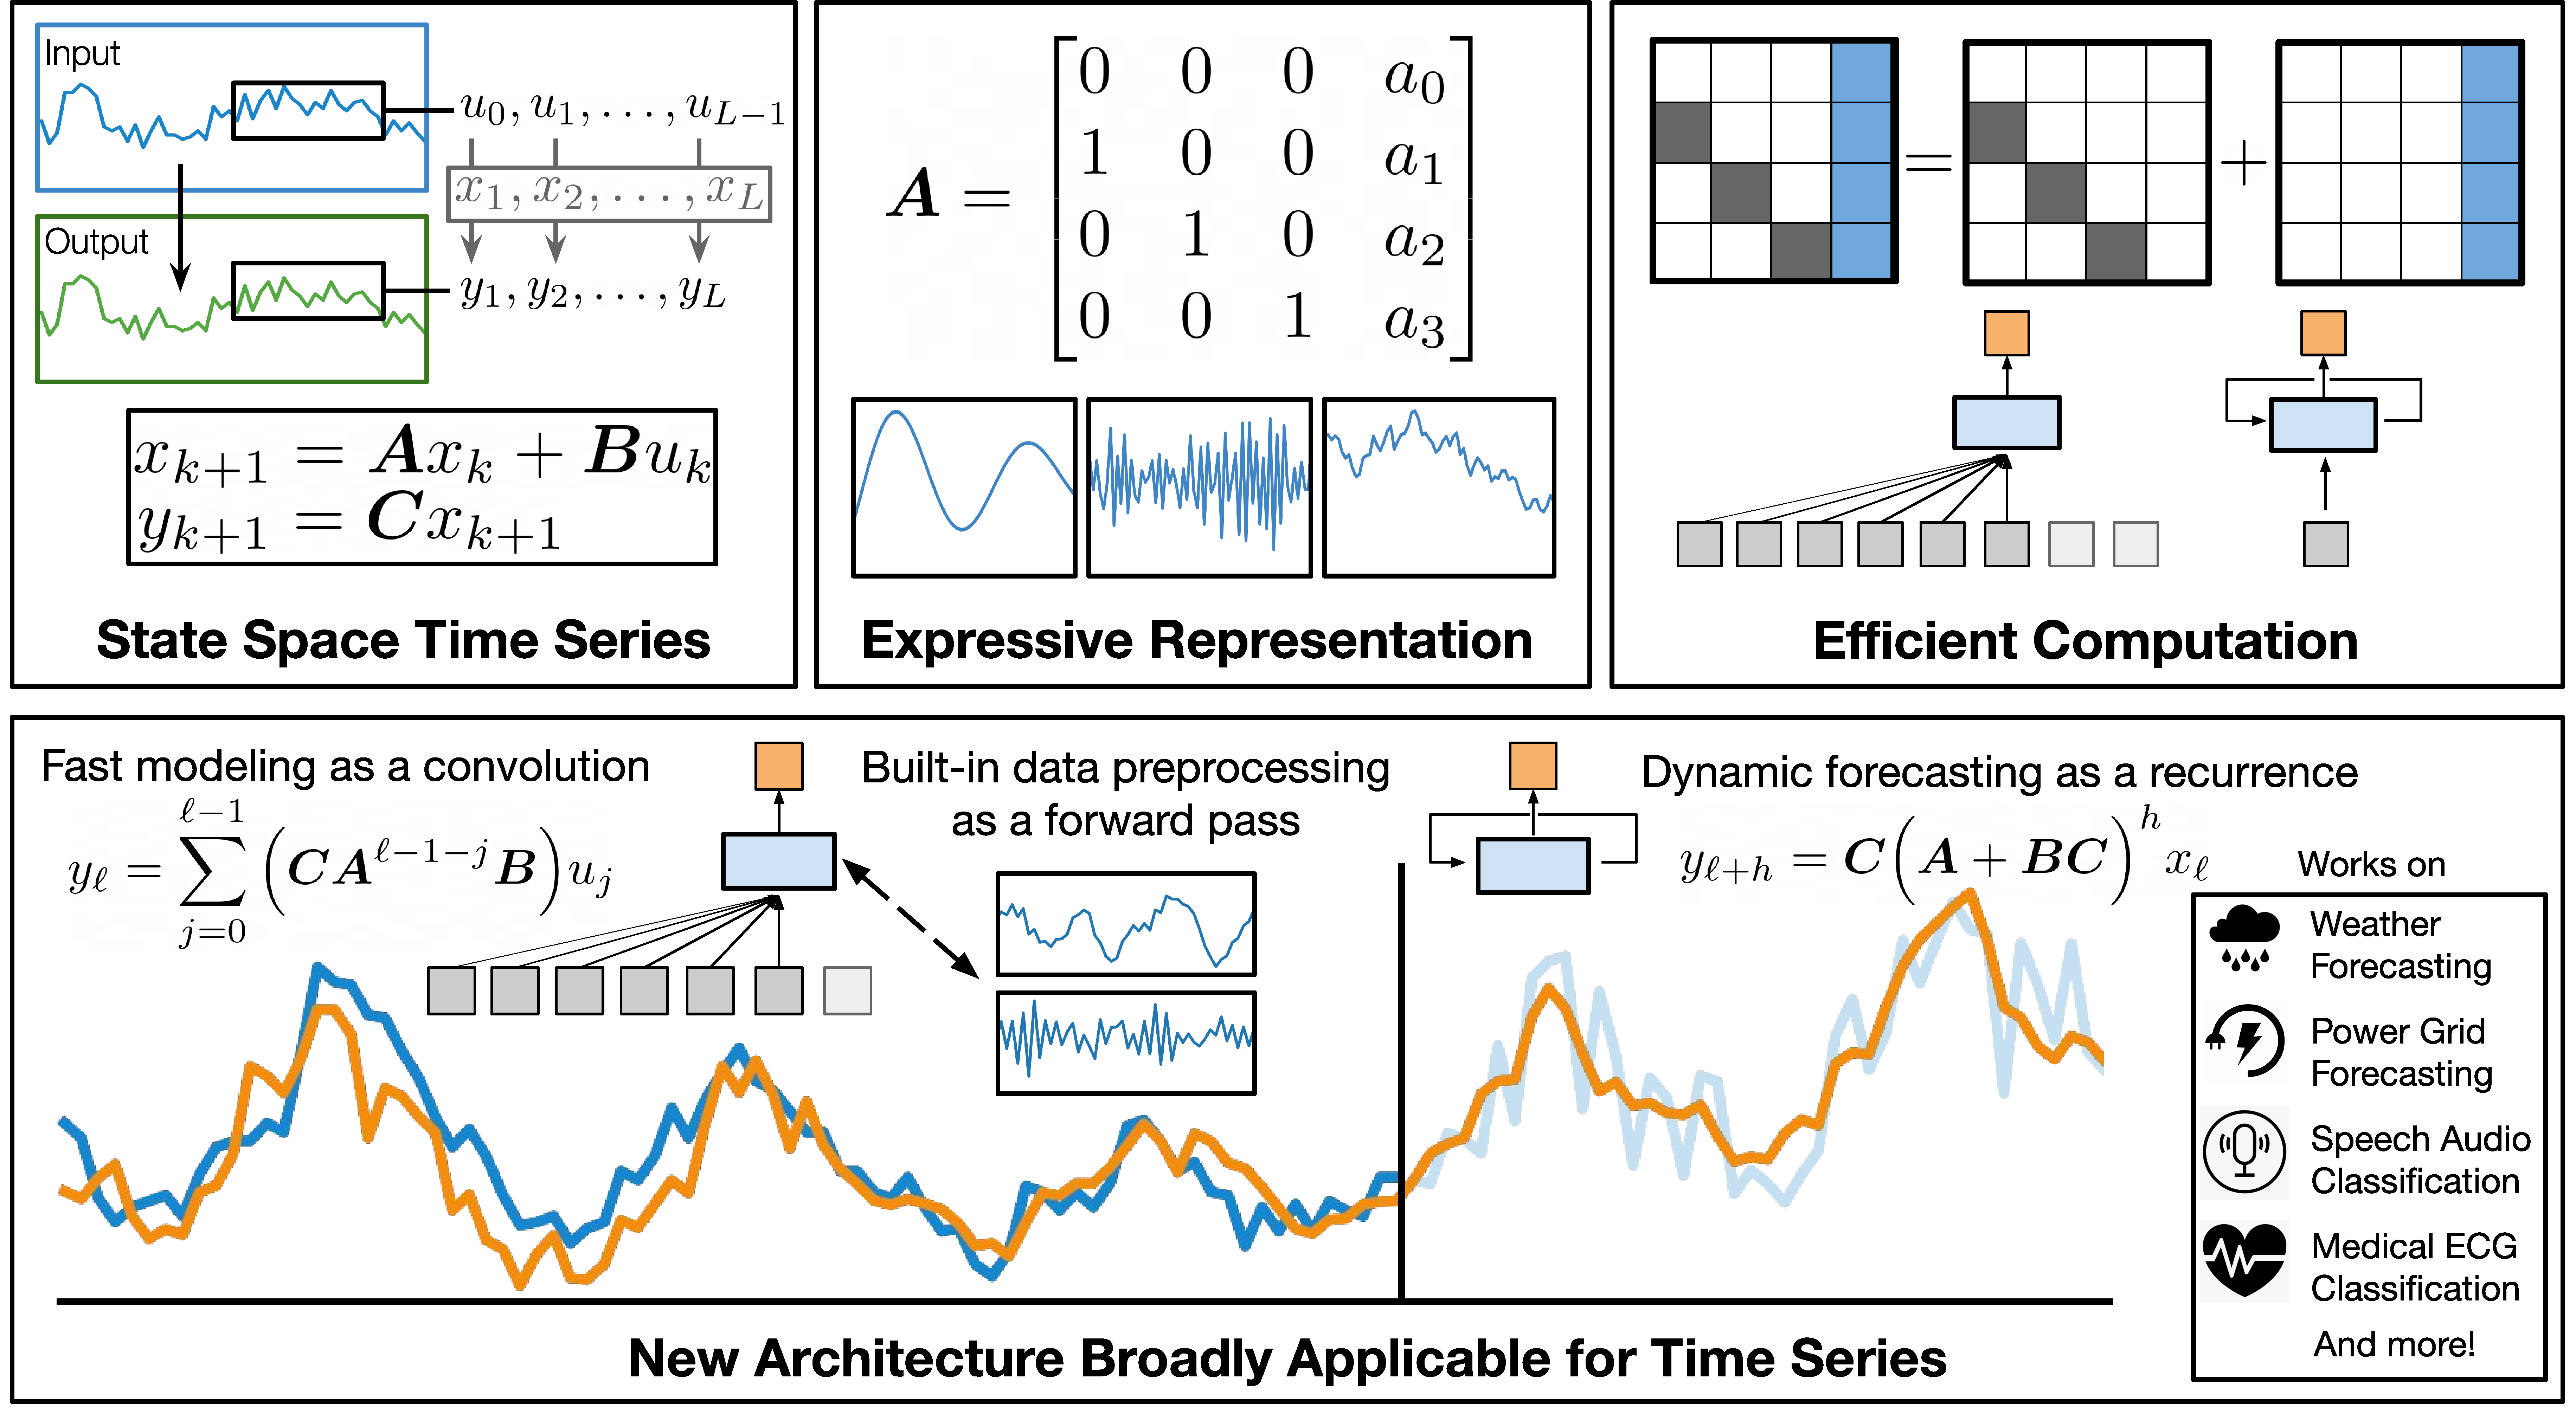
\includegraphics[width=1\textwidth]{_ICLR2023_paper/figures/time_series_ssm_use_this_2_levels_refactor1.pdf}
 \caption{We learn time series processes as state-space models (SSMs) (\textbf{top left}). We represent SSMs with the \textit{companion matrix}, which is a highly expressive representation for discrete time series  (\textbf{top middle}), and compute such SSMs efficiently as convolutions or recurrences via a shift + low-rank decomposition (\textbf{top right}). We use these SSMs to build \ourmethod{}, a new time series architecture broadly effective across tasks and domains (\textbf{bottom}).}
  \label{fig:overvew_fig1}
\end{figure}

% Our Method
%
% We thus propose \textbf{\ourmethod{}}, a new deep learning time series architecture. 
%
% Towards more effective time series modeling, 



We thus propose \textbf{\textsc{SpaceTime}}, a deep state-\textbf{space} architecture for effective \textbf{time} series modeling. 
% For more accurate forecasting and classification, 
To achieve this,
we focus on improving each criteria via three core contributions:

% \begin{enumerate}[itemsep=0.1pt,topsep=0pt,leftmargin=*]
\begin{enumerate}[topsep=0pt,leftmargin=*]
    \item For expressivity, our key idea and building block is a linear layer that models time series processes as \emph{state-space models} (SSMs) via the \emph{companion matrix} (Fig.~\ref{fig:overvew_fig1}). 
    We start with SSMs due to their connections to both classical time series analysis~\citep{kalman1960new, hamilton1994state} and recent deep learning advances~\citep{gu2021efficiently}. Classically, many time series models such as ARIMA and exponential smoothing (ETS) can be expressed as SSMs~\citep{box1970time, winters1960forecasting}. 
    Meanwhile, recent state-of-the-art deep sequence models~\citep{gu2021efficiently} have used SSMs to outperform Transformers and LSTMs on challenging long-range benchmarks~\citep{tay2020long}.
    % Meanwhile, recent SSM-based deep learning models~\citep{gu2021efficiently} have achieved state-of-the-art sequence modeling on challenging long-range benchmarks~\citep{tay2020long}. 
    Their primary innovations show how to formulate SSMs as neural network parameters that are practical to train. However, we find limitations with these deep SSMs for time series data. While we build on their advances, we prove that these prior SSM representations~\citep{ gu2021combining, gu2021efficiently, gupta2022diagonal}
    % cite these later: rangapuram2018, salinas2020deepar, lin2021ssdnet,
    cannot capture autoregressive processes fundamental for time series. We thus specifically propose the companion matrix representation for its expressive and memory-efficient properties. 
    We prove that the companion matrix SSM recovers fundamental autoregressive (AR) and smoothing processes modeled in classical techniques such as ARIMA and ETS, while only requiring $\mathcal{O}(d)$ memory to represent an $\mathcal{O}(d^2)$ matrix. 
    Thus, \ourmethod{} inherits the benefits of prior SSM-based sequence models, while introducing improved expressivity that 
    recovers fundamental time series processes
    % apture multiple AR processes and data preprocessing techniques 
    simply through its layer weights. 
    
    \item 
    % For forecasting over long horizons, we introduce a new ``closed-loop'' view of SSMs. Previous architectures apply the SSM in an ``open-loop'' fashion \citep{gu2021efficiently}, where the output is driven by the input sequence. 
    % However, to continuously forecast to long horizons, we require that the SSM has the ability to continue forecasting the signal in the absence of an input at those time steps. 
    % Inspired by classical closed-loop control~\citep{doyle2013feedback,aastrom2021feedback}, we propose a new variant of SSMs that explicitly models the next time-step input, which enables a multi-layer \ourmethod{} network to recurrently output long horizons.
    For forecasting long horizons, we introduce a new ``closed-loop'' view of SSMs. Prior deep SSM architectures either apply the SSM as an ``open-loop'' \citep{gu2021efficiently}, where fixed-length inputs necessarily generate same-length outputs, or use closed-loop autoregression where final layer outputs are fed through the \emph{entire} network as next-time-step inputs~\citep{goel2022s}. 
    We describe issues with both approaches in Sec.~\ref{sec:forecasting_ssm}, and instead achieve autogressive forecasting in a deep network with only a single SSM layer. We do so by explicitly training the SSM layer to predict its next time-step \emph{inputs}, alongside its usual outputs. This allows the SSM to recurrently generate its own future inputs that lead to desired outputs---\ie{} those that match an observed time series---so we can forecast over many future time-steps without explicit data inputs. 
    % This allows \ourmethod{} to generate its own final-layer inputs for outputting forecasts over many future time-steps.

    \item For efficiency, we introduce an algorithm for efficient training and inference with the companion matrix SSM. We 
    % first show how the companion SSM can be computed as both a convolution and a recurrence for layer-wise forward passes and forecasting respectively.  
    exploit the companion matrix's structure as a ``shift plus low-rank'' matrix, which allows us to reduce the time and space complexity for computing SSM hidden states and outputs from $\tilde{\mathcal{O}}(d \ell )$ to $\tilde{\mathcal{O}}(d + \ell)$ in SSM state size $d$ and input sequence length $\ell$. 
\end{enumerate}
% To subsequently build a full \ourmethod{} model, we simply stack together multiple layers---which each parametrize multiple companion matrix SSMs---into  a standard encoder-decoder architecture. 

% Simply stacking these layers together into a standard encoder-decoder architecture thus builds a highly expressive and efficient time series model.

In experiments, 
% we evaluate \ourmethod{} on extensive time series forecasting and classification tasks, and test if \ourmethod{}'s contributions empirically lead to (1) expressive time series modeling, (2) long-horizon forecasting, and (3) efficient training. 
%
we find \ourmethod{} consistently obtains state-of-the-art or near-state-of-the-art results, achieving best or second-best AUROC on 6 out of 7 ECG and audio speech time series classification tasks, and best mean-squared error (MSE) on 14 out of 16 Informer benchmark forecasting tasks~\citep{zhou2021informer}. \ourmethod{} also sets a new best average ranking across \numberMonashTasks{} tasks on the Monash benchmark~\citep{godahewa2021monash}.  
% 
We connect these gains with improvements on our three effective time series modeling criteria.  %
For expressivity, on synthetic ARIMA processes \ourmethod{} learns AR processes that prior deep SSMs cannot. 
%
% via extensive synthetics. As a controlled benchmark for expressiveness, we test how well popular architectures can fit standard AR processes, and find that \ourmethod{} best learns the true time series processes via its companion matrix SSM.
% compared to prior deep SSM representations.
%via visualizations of the process's ground-truth transfer function versus those parameterized by the trained SSM weights.
%
%
For long horizon forecasting, \ourmethod{} consistently outperforms prior state-of-the-art on the longest horizons by large margins. \ourmethod{} also generalizes better to \emph{new} horizons not used for training.
%
% validate that 
% We then validate (2) by showing that trained \ourmethod{}s generalize better to new horizons that models were not trained for. We also find that on the Informer benchmark, \ourmethod{} consistently outperforms alternatives on the longest evaluation horizons by the largest margins, up to $\textbf{X}$\% relative reduction in MSE for forecasting $\textbf{Y}$ time-steps.
%
% best RMSE on 25 out of 30 tasks from the diverse Monash benchmark~\citep{godahewa2021monash}.
% setting a new record among prior classical and deep learning approaches. 
% Moreover, we find that \ourmethod{} improves forecasts to arbitrary horizons (that it was not trained on) by \%XX on the Informer benchmark. 
For efficiency, on speed benchmarks \ourmethod{} obtains 73\% and 80\% relative wall-clock speedups over parameter-matched Transformers and LSTMs respectively, when training on real-world ETTh1 data.


\section{Regularization of Deep Neural Networks}
\label{sec:kernel_reg}
%!TEX root = main.tex

In this section, we recall the kernel perspective on deep networks introduced
by~\citet{bietti2018group}, and present upper and lower bounds on the RKHS norm
of a given model, leading to various regularization strategies.  For
simplicity, we first consider real-valued networks and binary classification,
before discussing multi-class extensions.

\subsection{Relation between deep networks and RKHSs}
\label{sub:rkhs_construction}
Kernel methods consist of mapping data living in a set~$\Xcal$ to a
RKHS~$\Hcal$ associated to a positive definite kernel~$K$ through a mapping
function $\Phi: \Xcal \to \Hcal$, and then learning simple machine learning
models in~$\Hcal$. Specifically, when considering a real-valued regression or
binary classification problem, classical kernel methods find a prediction
function $f : \mathcal{X} \to \R$ living in the RKHS which can be written in linear
form, i.e., such that $f(x) = \langle f, \Phi(x) \rangle_\Hc$ for all~$x$
in~$\Xcal$.  While explicit mapping to a possibly infinite-dimensional space is
of course only an abstract mathematical operation, learning~$f$ can be done
implicitly by computing kernel evaluations and typically by using convex
programming~\citep{scholkopf2001learning}.

Moreover, the RKHS norm~$\|f\|_\Hc$ acts as a natural regularization function,
which controls the variations of model predictions
according to the geometry induced by~$\Phi$:
\begin{equation}
\label{eq:cs}
|f(x) - f(x')| \leq \|f\|_\Hc \cdot \|\Phi(x) - \Phi(x') \|_\Hc.
\end{equation}
Unfortunately, our setup does not allow us to use the RKHS norm in a traditional way since evaluating the kernel is intractable. Instead, we
propose a different approach that considers explicit parameterized
representations of functions contained in the RKHS, given by generic CNNs,
and leverage properties of the RKHS and the
kernel mapping in order to regularize when learning the network parameters.


Consider indeed a real-valued deep convolutional network $f : \mathcal{X} \to
\R$, where $\mathcal X$ is simply $\R^d$, with rectified linear unit (ReLU) activations and no bias units.
By constructing an appropriate multi-layer hierarchical kernel, \citet{bietti2018group} show
that the corresponding RKHS~$\Hc$ contains a CNN with the same architecture and parameters as~$f$,
but with activations that are smooth approximations of ReLU.
Although the model predictions might not be strictly equal, we will abuse notation and denote this
approximation with smooth ReLU by~$f$ as well,
with the hope that the regularization procedures derived from the RKHS model
will be effective in practice on the original CNN~$f$.

Besides, the mapping~$\Phi(\cdot)$ is shown to be non-expansive:
\begin{equation}
\label{eq:non_expansive}
\|\Phi(x) - \Phi(x') \|_\Hc \leq \|x - x'\|_2,
\end{equation}
so that controlling~$\|f\|_\Hc$ provides some robustness to additive $\ell_2$-perturbations, by~\eqref{eq:cs}.
Additionally, with appropriate pooling operations, \citet{bietti2018group} show that the kernel mapping is also
stable to deformations, meaning that the RKHS norm also controls robustness to translations
and other transformations including scaling and rotations,
which can be seen as deformations when they are small.

In contrast to standard kernel methods, where the RKHS norm is typically available in closed form, this norm is difficult to compute in our setup, and requires approximations.
The following sections present upper and lower bounds on~$\|f\|_{\Hcal}$,
with linear convolutional operations denoted by~$W_k$ for $k=1, \ldots, L$, where~$L$ is the number of layers.
Defining~$\theta := \{W_k : k = 1, \ldots, L\}$, we then leverage these bounds to approximately solve the following
penalized or constrained optimization problems on a training set~$(x_i, y_i), i = 1, \ldots, n$:
\begin{align}
\label{eq:penalty_or_constraint}
& \min_\theta \frac{1}{n} \sum_{i=1}^n \ell(y_i, f_\theta(x_i)) + \lambda \|f_\theta\|_\Hc^2 \quad \text{or } \\
& \min_{\theta: \|f_\theta\|_\Hc \leq C} \frac{1}{n} \sum_{i=1}^n \ell(y_i, f_\theta(x_i)).
\end{align}
We also note that while the construction of~\citet{bietti2018group} considers VGG-like networks~\citep{simonyan2014very},
the regularization algorithms we obtain in practice can be easily adapted to different architectures
such as residual networks~\citep{he2016deep}.

\subsection{Exploiting lower bounds of the RKHS norm}
\label{sub:lower_bounds}

In this section, we devise regularization algorithms by leveraging lower bounds on~$\|f\|_\Hc$,
obtained by relying on the following variational characterization of Hilbert norms:
\begin{equation*}
\|f\|_\Hc = \sup_{\|u\|_\Hc \leq 1} \langle f, u \rangle_\Hc.
\end{equation*}
At first sight, this definition is not useful since the set $U = \{u \in \Hc : \|u\|_\Hc \leq 1\}$ may be 
infinite-dimensional
 and the inner products $\langle f, u \rangle_\Hc$ cannot be
computed in general. Thus, we devise tractable lower bound approximations by considering smaller sets~$\bar{U} \subset U$.

\paragraph{Adversarial perturbation penalty.}
Thanks to the non-expansiveness of $\Phi$, we can consider the subset $\bar U \subset U$ defined as $\bar{U} = \{\Phi(x + \delta) - \Phi(x) : x \in \mathcal X, \|\delta\|_2 \leq 1 \}$,
leading to the bound
\begin{equation}
\label{eq:lower_bound}
\|f\|_\Hc  \geq  \|f\|_\delta^2 := \sup_{x \in \mathcal X, \|\delta\|_2 \leq 1} f(x + \delta) - f(x),
\end{equation}
which is reminiscent of adversarial perturbations. Adding a regularization parameter $\epsilon > 0$ in front of the norm
then corresponds to different sizes of perturbations:
\begin{equation}
\label{eq:kernel_adv}
\epsilon \|f\|_\Hc = \sup_{\|u\|_\Hc \leq \epsilon} \langle f, u \rangle_\Hc \geq \sup_{x \in \mathcal X, \|\delta\|_2 \leq \epsilon} f(x + \delta) - f(x).
\end{equation}
Using this lower bound or its square as a penalty in the objective~\eqref{eq:penalty_or_constraint}
when training a CNN provides a way to regularize.
Optimizing over adversarial perturbations has been useful to obtain robust models~\citep[\eg, the PGD method of~][]{madry2018towards};
yet our approach differs in two important ways: 

(i) it involves a penalty that is decoupled from the loss term such that 
in principle, our penalty could be used beyond the supervised empirical risk paradigm.
In contrast, PGD optimizes the robust formulation~\eqref{eq:robust} below, which 
fits training data while considering
perturbations on the loss.

(ii) our penalty involves a global maximization problem
on the input space~$\Xcal$, as opposed to only maximizing on perturbations near
training data. In practice, optimizing over~$\Xcal$ is however
difficult and instead, we replace~$\Xcal$ by random mini-batches of examples,
yielding further lower bounds on the RKHS norm. These examples may be labeled or not,
in contrast to PGD that perturb labeled examples only.
When using such a mini-batch,
a gradient of the penalty can be obtained by first finding maximizers~$\hat x, \hat \delta$
(where~$\hat x$ is an element of the mini-batch and $\hat{\delta}$ is a perturbation), and then computing gradients
of $f_\theta(\hat x + \hat \delta) - f_\theta(\hat x)$ with respect to~$\theta$ by using back-propagation.
In practice, we compute the perturbations~$\delta$ for each example~$x$ by using a few steps of
projected gradient ascent with constant step-lengths.

\paragraph{Robust optimization yields another lower bound.}
In some contexts, our penalized approach is related to solving the robust optimization problem
\begin{equation}
\label{eq:robust}
\min_\theta \frac{1}{n} \sum_{i=1}^n \sup_{\|\delta\|_2 \leq \epsilon} \ell(y_i, f_\theta(x_i + \delta)),
\end{equation}
which is commonly considered for training adversarially robust classifiers~\citep{wong2018provable,madry2018towards,raghunathan2018certified}.
In particular, \citet{xu2009robustness} show that the penalized and
robust objectives are equivalent in the case of the hinge loss with linear predictors,
when the data is non-separable.
They also show the equivalence for kernel methods when considering the (intractable) full perturbation set~$U$
around each point in the RKHS~$\Phi(x_i)$, that is, predictions $\langle f, \Phi(x_i) + u \rangle_\Hc$ with~$u$ in $U$.
Intuitively, when a training example $(x_i, y_i)$ is misclassified, we are in the ``linear'' part of the hinge loss, such~that
\begin{equation*}
\sup_{\|u\|_\Hc \leq \epsilon} \ell(y_i, \langle f, \Phi(x_i) + u \rangle_\Hc) = \ell(y_i, f(x_i)) + \epsilon \|f\|_{\Hcal}.
\end{equation*}
For other losses such as the logistic loss, a regularization effect is still present even
for correctly classified examples,
though it may be smaller since the loss has a reduced slope for such points.
This leads to an \emph{adaptive} regularization mechanism that may automatically reduce
the amount of regularization when the data is easily separable.
However, the robust optimization approach might only encourage local stability around training examples, while the global quantity~$\|f\|_\Hc$
may become large in order to better fit the data.
We note that a perfect fit of the data with large complexity does not prevent generalization~\citep[see, \eg,][]{belkin2018overfitting,belkin2018understand};
yet, such mechanisms are still poorly understood.
Nevertheless, it is easy to show that the robust objective~\eqref{eq:robust}
lower bounds the penalized objective with penalty~$\epsilon \|f\|_{\Hcal}$.

\paragraph{Gradient penalties.}
Taking $\bar{U} \!= \! \{\frac{\Phi(x) - \Phi(y)}{\|x - y\|_2} : x, y \!\in\! \mathcal X\}$, which is a subset of~$U$
by Eq.~\eqref{eq:non_expansive}---it turns out that this is the same set as for adversarial perturbation penalties,
since~$\Phi$ is homogeneous~\citep{bietti2018group} and $\mathcal X =
\Real^d$---we obtain a lower bound based on the Lipschitz constant of~$f$:
\begin{equation}
\|f\|_\Hc \geq \sup_{x, y \in \mathcal{X}} \frac{f(x) - f(y)}{\|x - y\|_2} \geq \|\nabla f\| := \sup_{x \in \mathcal X} \|\nabla f(x)\|_2, \label{eq:gradientpenalty}
\end{equation}
where the second inequality becomes an equality when~$\Xcal$ is convex,
and the supremum is taken over points where~$f$ is differentiable.
Although we are unaware of previous work using this exact lower bound for a generic regularization penalty,
we note that variants replacing the supremum over~$x$ by an expectation over data have been recently used
to stabilize the training of generative adversarial networks~\citep{gulrajani2017improved,roth2017stabilizing},
and we provide insights in Section~\ref{sub:gan_reg} on the benefits of RKHS regularization in such a setting.
Related penalties have been considered in the context of robust optimization,
for regularization or robustness,
noting that a penalty based on the gradient of the loss function $x \mapsto \ell(y, f(x))$ can give a good approximation of~$\eqref{eq:robust}$
when~$\epsilon$ is small~\citep{drucker1991double,lyu2015unified,roth2018adversarially,simon2018adversarial}.

\paragraph{Penalties based on deformation stability.}
We may also obtain new penalties by considering more exotic sets
$\bar{U} = \{\Phi(\tilde x) - \Phi(x) : x~\in~{\mathcal X},~ \tilde x \text{ is a small} \text{ deformation of }x\}$,
where the amount of deformation is dictated by the stability bounds of~\citet{bietti2018group} in order to ensure that $\bar{U} \subset U$.
More precisely, such bounds depend on the maximum displacement and Jacobian norm of
the diffeomorphisms considered. These can be easily computed for various parameterized families
of transformations, such as translations, scaling or rotations, leading to simple ways to control
the regularization strength through the parameters of these transformations.
One can also consider infinitesimal deformations from such parameterized transformations,
which approximately yields the \emph{tangent propagation} regularization
strategy of~\citet{simard1998transformation}.
These approaches are detailed in Appendix~\ref{sec:deformation_penalties}.
If instead we consider the robust optimization formulation~\eqref{eq:robust}, we obtain a form
of \emph{data augmentation} where transformations are optimized instead of sampled, as done by~\citep{engstrom2017rotation}.


\paragraph{Extensions to multiple classes and beyond}
\label{sub:multiclass}

We now extend the regularization strategies based on lower bounds to multi-valued networks,
in order to deal with multiple classes.
For that purpose, we consider a multi-class penalty $\|f_1\|_\Hc^2 + \ldots + \|f_K\|_\Hc^2$
for an~$\R^K$-valued function $f = (f_1, f_2, \ldots, f_K)$, and we define 
\begin{align*}
\|f\|_\delta^2 := \sum_{k=1}^K \|f_k\|_\delta^2 \text{~~~and~~~} \|\nabla f\|^2 := \sum_{k=1}^K \|\nabla f_k\|^2,
\end{align*}
where $\|f_k\|_\delta$ is the adversarial penalty~(\ref{eq:lower_bound}), and $\|\nabla f_k\|$ is defined in~(\ref{eq:gradientpenalty}).
For deformation stability penalties, we proceed in a similar manner,
and for robust optimization formulations~\eqref{eq:robust}, the extension is straightforward,
given that multi-class losses such as cross-entropy can be
directly optimized in an adversarial training or gradient penalty setup.

Finally, we note that while the kernel approach we introduce considers
the Euclidian geometry in the input space, it is possible to consider heuristic alternatives for other
geometries, such as~$\ell_\infty$ perturbations, as discussed in Appendix~\ref{sec:non_euclidian_appx}.

\subsection{Exploiting upper bounds with spectral norms}
\label{sub:upper_bounds}

Instead of lower bounds, one may use instead
 the following upper bound from~\citet[Proposition 14]{bietti2018group}:
\begin{equation}
\label{eq:upper_bound}
\|f\|_\Hc \leq \omega(\|W_1\|, \ldots, \|W_L\|),
\end{equation}
where~$\omega$ is increasing in all of its arguments, and~$\|W_k\|$ is the spectral norm of the linear
operator~$W_k$.
Here, we simply consider the spectral norm on the filters, given by~$\|W\| := \sup_{\|x\|_2 \leq 1} \|W x\|_2$.
Other generalization bounds relying on similar quantities have been proposed for
controlling complexity~\citep{bartlett2017spectrally,neyshabur2017pac}, suggesting that using them for
regularization is relevant even beyond our kernel perspective,
as observed by~\citet{cisse2017parseval,sedghi2018singular,yoshida2017spectral}.
Extensions to multiple classes are simple to obtain by simply considering spectral norms up to
the last layer.


\paragraph{Penalizing the spectral norms.}
One way to control the upper bound~\eqref{eq:upper_bound} when learning a neural network~$f_\theta$
is to consider a regularization penalty based on spectral norms
\begin{equation} 
	\label{eq:optimization_problem_penalized} 
	\min_{\theta}\frac{1}{n} \sum_{i=1}^{n} \ell(y_i, f_{\theta}(x_i)) + \lambda \sum_{l=1}^{L} \|W_l\|^2,
\end{equation}
where~$\lambda$ is a regularization parameter.
To optimize this cost, one can obtain (sub)gradients of the penalty by computing singular vectors
associated to the largest singular value of each~$W_l$.
We consider the method of~\citet{yoshida2017spectral}, which computes such singular vectors approximately
using one or two iterations of the power method, as well as a more costly approach using the full SVD.

\paragraph{Constraining the spectral norms with a continuation approach.}
In the constrained setting, we want to optimize:
\begin{equation*}
\begin{aligned}
\min_{\theta}\frac{1}{n} \sum_{i=1}^{n} \ell(y_i, f_{\theta}(x_i)) \text{~~s.t.~~} \|W_l\| \leq \tau \text{ ; } l\in 1, \dots, L~,
\end{aligned}
\end{equation*}
where $\tau$ is a user-defined constraint.
This objective may be optimized by projecting each~$W_l$ in the
spectral norm ball of radius $\tau$ after each gradient step.
Such a projection is achieved by truncating the singular values to be smaller than~$\tau$ (see Appendix~\ref{sec:spectral_norms_appx}).
We found that the loss was hardly optimized with this approach,
and therefore introduce a continuation approach with an exponentially
decaying schedule for~$\tau$ reaching a constant $\tau_0$
after a few epochs, which we found to be important for good empirical performance.

\subsection{Combining upper and lower bounds.}
One advantage of lower bound penalties is that they are independent of
the model parameterization, making them flexible enough to use with more complex architectures.
In addition, the connection with robust optimization can provide a useful mechanism for adaptive regularization.
However, they do not provide a guaranteed control on the RKHS norm, unlike the upper bound strategies.
This is particularly true for robust optimization approaches, which may favor small training loss
and local stability over global stability through~$\|f\|_\Hc$.
Nevertheless, we observed that our new approaches based on separate penalties
sometimes do help in controlling upper bounds as well (see Section~\ref{sec:experiments}).

While these upper bound strategies are useful for limiting model complexity,
we found them empirically less effective for robustness (see Section~\ref{sub:exp_robust}).
However, we observed that combining with lower bound approaches can overcome this weakness,
perhaps due to a better control of local stability.
In particular, such combined approaches often provide the best generalization performance
in small data scenarios, as well as better guarantees on adversarially robust generalization
thanks to a tighter control of the RKHS norm.



\section{Theoretical Guarantees and Insights}
\label{sec:theory}
%!TEX root = main.tex

In this section, we study how the kernel perspective allows us to extend standard margin-based generalization bounds 
to an adversarial setting in order to
provide theoretical guarantees on adversarially robust generalization.
We then discuss how our kernel approach provides novel interpretations for training
generative adversarial networks.

\subsection{Guarantees on adversarial generalization}
\label{sub:guarantees}

While various methods have been introduced to empirically gain robustness to adversarial perturbations,
the ability to generalize with such perturbations, also known as \emph{adversarial generalization}~\citep{schmidt2018adversarially},
still lacks theoretical understanding.
Margin-based bounds have been useful
to explain the generalization behavior of learning algorithms that can fit the training data
well, such as kernel methods, boosting and neural networks~\citep{koltchinskii2002empirical,boucheron2005theory,bartlett2017spectrally}.
Here, we show how such arguments can be adapted to obtain guarantees on adversarial generalization,
\ie, on the expected classification error in the presence of an~$\ell_2$-bounded adversary,
based on the RKHS norm of a learned model.
For a binary classification task with labels in $\mathcal Y = \{-1,1\}$ and data distribution~$\mathcal D$,
we would like to bound the expected adversarial error of a classifier~$f$, given for some $\epsilon > 0$ by
\begin{equation}
\label{eq:adv_error}
\text{err}_\mathcal D(f, \epsilon) := P_{(x,y) \sim \mathcal D} (\exists \|\delta\|_2 \leq \epsilon: ~y f(x + \delta) < 0).
\end{equation}
Leveraging the fact that~$f$ is $\|f\|_\Hc$-Lipschitz,
we now show how to further bound this quantity using empirical margins,
following the usual approach to obtaining margin bounds for kernel methods~\citep[\eg,][]{boucheron2005theory}.
Consider a training dataset $(x_1, y_1), \ldots, (x_n, y_n) \in \mathcal X \times \mathcal Y$.
Defining $L_n^\gamma(f) := \frac{1}{n} \sum_{i=1}^n \textbf{1}\{y_i f(x_i) < \gamma\}$,
we have the following bound, proved in Appendix~\ref{sec:generalization_appx}:
\begin{proposition}[Adversarially robust margin bound]
\label{prop:robust_margin_bound}
With probability~$1 - \delta$ over a dataset $\{(x_i, y_i)\}_{i=1, \ldots, n}$, we have,
for all choices of $\gamma > 0$ and~$f \in \Hc$,
\begin{align}
\label{eq:robust_margin_bound}
& \text{err}_\mathcal D(f, \epsilon) \leq L_n^{\gamma + 2 \epsilon \|f\|_\Hc}(f) + \tilde{O}\left( \frac{\|f\|_\Hc \bar{B}}{\gamma \sqrt{n}}  \right),
\end{align}
where $\bar{B} = \sqrt{\frac{1}{n}\sum_{i=1}^n K(x_i, x_i)}$ and $\tilde{O}$ hides a term depending logarithmically on~$\|f\|_\Hc, \gamma$, and $\delta$.
\end{proposition}

When $\epsilon = 0$, we obtain the usual margin bound, while $\epsilon > 0$ yields
a bound on adversarial error~$\text{err}_\mathcal D(f, \epsilon)$,
for some neural network~$f$ learned from data.
Note that other complexity measures based on products of spectral norms may be used instead of~$\|f\|_\Hcal$,
as well as multi-class extensions, following~\citet{bartlett2017spectrally,neyshabur2017pac}.
In concurrent work, \citet{khim2018adversarial,yin2019rademacher} derive similar bounds
in the context of fully-connected networks.
In contrast to these works, which bound complexity of a modified function class,
our bound uses the complexity of the original class and leverages smoothness properties
of functions to derive the margin bound.

One can then study the effectiveness of a regularization algorithm by inspecting
cumulative distribution (CDF) plots of the
\emph{normalized margins} $\bar{\gamma}_i = y_i f(x_i) / \|f\|_\Hc$,
for different strengths of regularization (an example is given in Figure~\ref{fig:norms_and_margins}, Section~\ref{sub:exp_robust}).
According to the bound~\eqref{eq:robust_margin_bound}, one can assess expected adversarial error with $\epsilon$-bounded perturbations
by looking at the part of the plot to the right of~$\bar{\gamma} = 2\epsilon$.
In particular, the value of the CDF at such a value of~$\bar{\gamma}$ is representative of the
bound for large~$n$ (since the second term is negligible),
while for smaller~$n$, the best bound is obtained for a larger value of~$\bar{\gamma}$, which also suggests that
the right side of the plots is indicative of performance on small datasets.

When the RKHS norm can be well approximated, our bound provides a certificate on
test error in the presence of adversaries. 
While such an approximation is difficult to
obtain in general, the guarantee is most useful when lower and upper bounds of the RKHS norm are controlled together.


\subsection{New insights on generative adversarial networks}
\label{sub:gan_reg}

Generative adversarial networks (GANs) attempt to learn a \emph{generator} neural network~$G_\phi : \mathcal Z \to \mathcal X$,
so that the distribution of~$G_\phi(z)$ with~$z \sim D_z$ a noise vector resembles a data distribution~$D_x$.
In this section, we discuss connections between recent regularization techniques for
training GANs, and approaches to learning generative models
based on a MMD criterion~\citep{gretton2012kernel}, in view of our RKHS framework.
Our goal is to provide a new insight on these methods, but not necessarily to provide a new one.

Various recent approaches have relied on regularization strategies on a \emph{discriminator} network
in order to improve the stability of GAN training and the quality of the produced samples.
Some of these resemble the approaches presented in Section~\ref{sec:kernel_reg}
such as gradient penalties~\citep{gulrajani2017improved,roth2017stabilizing}
and spectral norm regularization~\citep[]{miyato2018spectral}.
We provide an RKHS interpretation of these methods as
optimizing an MMD distance with the convolutional kernel introduced in Section~\ref{sec:kernel_reg}:
\begin{equation}
\label{eq:ckn_mmd}
\min_\phi \sup_{\|f\|_\Hc \leq 1} \E_{x \sim D_x}[ f(x)] - \E_{z \sim D_z}[f(G_\phi(z))].
\end{equation}
When learning from an empirical distribution over~$n$ samples,
the MMD criterion is known to have much better sample complexity than the Wasserstein-1
distance considered by~\citet{arjovsky2017wasserstein} for high-dimensional data
such as images~\citep{sriperumbudur2012empirical}.
While the MMD approach has been used for training generative models, it generally relies on a generic kernel function,
such as a Gaussian kernel, that appears explicitly in the objective~\citep{dziugaite2015training,li2017mmd,binkowski2018demystifying}.
Although using a learned feature extractor can improve this, the Gaussian kernel might be a poor choice when
dealing with natural signals such as images, while the hierarchical kernel we consider in our paper is better suited
for this type of data, by providing useful invariance and stability properties.
Leveraging the variational form of the MMD~\eqref{eq:ckn_mmd} with this kernel suggests for instance using convolutional networks
as the discriminator~$f$, with constraints on the spectral norms in order to ensure~$\|f\|_\Hc \leq C$ for some~$C$,
as done by~\citet{miyato2018spectral} through normalization.


\section{Experiments}
\label{sec:experiments}
\vspace{-0.2cm}
\section{Experiments Details}
\label{sec:exp}

\vspace{-0.2cm}
\subsection{Roadmap Insights on FFHQ-256\texorpdfstring{~\cite{sg1}}{}}
\label{sub:arc-experiments}
\vspace{-0.1cm}
As per Table~\ref{tab:roadmap}, Config A (vanilla StyleGAN2) achieves an FID of 7.52 using the official implementation on FFHQ-256. Config B with all tricks removed achieves an FID of 12.46---performance drops as expected. 
Config C, with a well-behaved loss, achieves an FID of 11.65. But, now training is sufficiently stable to improve the architecture.

Config D, which improves $G$ and $D$ based on the classic ResNet and ConvNeXt findings, achieves an FID of 9.95. The output skips of the StyleGAN2 generator are no longer useful given our new architecture; including them produces a worse FID of 10.17. Karras~\etal find that the benefit of output skips is mostly related to gradient magnitude dynamics~\cite{sg3}, and this has been addressed by our ResNet architecture. For StyleGAN2, Karras~\etal conclude that a ResNet architecture is harmful to $G$~\cite{sg2}, but this is not true in our case as their ResNet implementation is considerably different from ours: 1) Karras~\etal use one 3-3 residual block for each resolution stage, while we have a separate transition layer and two 1-3-1 residual blocks; 2) i.3) and i.4) are violated as they do not have a linear residual block~\cite{mobnet} and the transition layer is placed on the skip branch of the residual block rather than the stem; 3) the essential principle of ResNet~\cite{resnet}---identity mapping~\cite{resnet2}---is violated as Karras~\etal divide the output of the residual block by $\sqrt{2}$ to avoid variance explosion due to the absence of a proper initialization scheme.

For Config E, we conduct two experiments that ablate i.\ref{item:i1} (increased width with depthwise conv.) and i.\ref{item:i2} (an inverted bottleneck). We add GroupedConv and reduce the bottleneck compression ratio to two given the same model size. Each bottleneck is now 1.5$\times$ the width of Config A, and the FID drops to 7.51, surpassing the performance of StyleGAN2. By inverting the stem and the bottleneck dimensions to enhance the capacity of GroupedConv, our final model achieves an FID of 7.05, exceeding StyleGAN2.


\begin{wraptable}[12]{r}{6.5cm}
\vspace{-1.25cm}
\centering
\caption{StackedMNIST 1000-mode coverage.}
% Our model outperforms other GANs in terms of $D_\text{KL}$, indicating that we are better able to recover the distribution.}
\vspace{-0.4cm}
\resizebox{0.8\linewidth}{!}{
\begin{tblr}{
  cell{2}{2} = {c},
  cell{2}{3} = {c},
  cell{3}{2} = {c},
  cell{3}{3} = {c},
  cell{4}{2} = {c},
  cell{4}{3} = {c},
  cell{5}{2} = {c},
  cell{5}{3} = {c},
  cell{6}{2} = {c},
  cell{6}{3} = {c},
  cell{7}{2} = {c},
  cell{7}{3} = {c},
  cell{8}{2} = {c},
  cell{8}{3} = {c},
  cell{9}{2} = {c},
  cell{9}{3} = {c},
  cell{10}{2} = {c},
  cell{10}{3} = {c},
  cell{11}{2} = {c},
  cell{11}{3} = {c},
  cell{12}{2} = {c},
  cell{12}{3} = {c},
  hline{2,12} = {1-3}{},
}
Model     & \# modes$\uparrow$ & $D_\text{KL}$$\downarrow$            &  \\
DCGAN~\cite{dcgan}     & 99            & 3.40\phantom{0}&  \\
VEEGAN~\cite{srivastava2017veegan}    & 150           & 2.95\phantom{0}&  \\
WGAN-GP~\cite{wgan-gp}& 959           & 0.73\phantom{0}&  \\
PacGAN~\cite{pacgan}    & 992           & 0.28\phantom{0}&  \\
StyleGAN2~\cite{sg2} & 940           & 0.42\phantom{0}&  \\
PresGAN~\cite{presgan}   & \textbf{1000} & 0.12\phantom{0}&  \\
Adv. DSM~\cite{advsm}  & \textbf{1000} & 1.49\phantom{0}&  \\
VAEBM~\cite{vaebm}     & \textbf{1000} & 0.087          &  \\
DDGAN~\cite{ddgan}     & \textbf{1000} & 0.071          &  \\
MEG~\cite{meg}       & \textbf{1000} & 0.031          &  \\
Ours---Config E     & \textbf{1000} & \textbf{0.029} &  
\end{tblr}
}
\label{tab:stackedmnist}
\end{wraptable}%

\subsection{Mode Recovery --- StackedMNIST\texorpdfstring{~\cite{metz2016unrolled}}{}} 
\vspace{-0.1cm}
We repeat the earlier experiment in 1000-mode convergence on StackedMNIST (unconditional generation), but this time with our updated architecture and with comparisons to SOTA GANs and likelihood-based methods (Tab.~\ref{tab:stackedmnist}, Fig.~\ref{fig:stacked-mnist}). 
One advantage brought up of likelihood-based models such as diffusion over GANs is that they achieve mode coverage~\cite{adm}. We find that most GANs struggle to find all modes. But, PresGAN~\cite{presgan}, DDGAN~\cite{ddgan}, and our approach are successful. Further, our method outperforms all other tested GAN models in term of KL divergence.

\subsection{FID --- FFHQ-256\texorpdfstring{~\cite{sg1}}{} (Optimized)}
\vspace{-0.1cm}
We train Config E model until convergence and with optimized hyperparameters and training schedule on FFHQ at 256$\times$256 (unconditional generation) (Tab.~\ref{tab:ffhq256}, Figs.~\ref{fig:ffhq-256-teaser} and~\ref{fig:ffhq-256}). 
Please see our supplemental material for training details.
%The hyperparameters and schedule are listed in the supplemental material. 
Our model outperforms existing StyleGAN methods, plus four more recent diffusion-based methods. On this common dataset experimental setting, many methods (not listed here) use the bCR~\cite{zhao2021improved} trick---this has only been shown to improve performance on FFHQ-256 (not even at different resolutions of FFHQ)~\cite{zhao2021improved, zhang2022styleswin}. We do not use this trick. 
% no such tricks in our method.
% JT Try to minimize embellishment...
% This is particularly impressive given the fact that the dataset FFHQ was designed for StyleGAN~\cite{sg1} and the StyleGAN series of models were optimized with this specific dataset in mind.
% to achieve this performance.

\subsection{FID --- FFHQ-64\texorpdfstring{~\cite{edm}}{}}
\vspace{-0.1cm}
To compare with EDM~\cite{edm} directly, we evaluate our model on FFHQ at 64$\times$64 resolution. For this, we remove the two highest resolution stages of our 256$\times$256 model, resulting in a generator that is less than half the number of parameters as EDM. Despite this, our model outperforms EDM on this dataset and needs one function evaluation only (Tab.~\ref{tab:ffhq64}).

\begin{figure}
\begin{floatrow}
    %\hspace{-0.75cm}%
    \capbtabbox{%
        \centering
        \resizebox{\linewidth}{!}{
        \begin{tblr}{
          column{2,3} = {r},
          cell{1}{2} = {c},
          cell{1}{3} = {c},
          hline{2,5,9,10} = {-}{},
        }
        Model       & NFE$\downarrow$ & FID$\downarrow$  \\
        StyleGAN2~\cite{sg2}   & 1               & 3.78 \\
        StyleGAN3-T~\cite{sg3} & 1               & 4.81 \\
        StyleGAN3-R~\cite{sg3} & 1               & 3.92 \\
        LDM~\cite{rombach2022high} & 200               & 4.98\\
        ADM (DDIM)~\cite{adm,compdiff} & 500               & 8.41\\
        ADM (DPM-Solver)~\cite{adm,compdiff} & 500               & 8.40\\
        Diffusion Autoencoder~\cite{diffae,compdiff} & 500               & 5.81\\
        Ours---Config E  & 1               & 2.75 \\
        \emph{With ImageNet feature leakage~\cite{kynkaanniemi2022role}:} & & \\
        PolyINR*~\cite{singh2023polynomial} & 1               & 2.72 \\
        StyleGAN-XL*~\cite{sgxl} & 1               & 2.19 \\
        StyleSAN-XL*~\cite{takida2024san} & 1               & 1.68 \\
        \end{tblr}
        }
    }{%
        \caption{
        \label{tab:ffhq256}FFHQ-256. * denotes models that leak ImageNet features.}
    }
    %
    \capbtabbox{%
        \centering
        \resizebox{0.85\linewidth}{!}{
        \begin{tblr}{
          column{2} = {r},
          column{3} = {r},
          hline{2,5,8} = {-}{},
        }
        Model         & NFE$\downarrow$ & FID$\downarrow$ \\
        StyleGAN2~\cite{sg2,anycostgan}     & 1               & 3.32            \\
        MSG-GAN~\cite{karnewar2020msg,anycostgan}       & 1               & 2.7             \\
        Anycost GAN~\cite{anycostgan}   & 1               & 2.52            \\
        VE~\cite{sde,edm}            & 79              & 25.95           \\
        VP~\cite{sde,edm}            & 79              & 3.39            \\
        EDM~\cite{edm}           & 79              & 2.39            \\
        Ours—Config E & 1               & 1.95 \\
        \end{tblr}
        }
    }{%
        \caption{\label{tab:ffhq64}FFHQ-64.}
    }
\end{floatrow}
\vspace{-0.25cm}
\end{figure}


% \begin{figure}
% \begin{floatrow}
%     \capbtabbox{%
%         \centering
%         \resizebox{0.8\linewidth}{!}{
%         \begin{tblr}{
%           column{2,3} = {r},
%           cell{1}{2} = {c},
%           cell{1}{3} = {c},
%           hline{2,9,13} = {-}{},
%         }
%         Model               & NFE$\downarrow$ & FID$\downarrow$ \\
%         BigGAN~\cite{biggan}              & 1               & 14.73 \\
%         TransGAN~\cite{trans}            & 1               & 9.26 \\
%         ViTGAN~\cite{vitgan}              & 1               & 6.66 \\
%         DDGAN~\cite{ddgan}               & 4               & 3.75 \\
%         Diffusion StyleGAN2~\cite{diffusiongan} & 1               & 3.19 \\
%         StyleGAN2 + ADA~\cite{sg2ada}     & 1               & 2.42 \\
%         StyleGAN3-R + ADA~\cite{sg3,studio}   & 1               & 10.83 \\
%         DDPM~\cite{ddpm}               & 1000            & 3.21 \\
%         DDIM~\cite{ddim}                & 50             & 4.67 \\
%         VE~\cite{sde,edm}                  & 35              & 3.11 \\
%         VP~\cite{sde,edm}                  & 35              & 2.48 \\
%         Ours---Config E     & 1               & 1.96 \\
%         \hline
%         \emph{With ImageNet feature leakage~\cite{kynkaanniemi2022role}:} & & \\
%         StyleGAN-XL*~\cite{sgxl}       & 1               & 1.85 \\
%         \end{tblr}
%         }
%     }{%
%         \caption{\label{tab:cifar10}CIFAR-10.}
%     }
%         % \begin{tblr}{
%         %   column{2,3} = {r},
%         %   cell{1}{2}{3} = {},
%         %   hline{2,9,13} = {-}{},
%         % }
%         % Model               & FID$\downarrow$ & Params          \\
%         % BigGAN~\cite{biggan}              & 14.73  & --       \\
%         % TransGAN~\cite{trans}            & 9.26 & --         \\
%         % ViTGAN~\cite{vitgan}              & 6.66 & --         \\
%         % DDGAN~\cite{ddgan}               & 3.75 & --         \\
%         % Diffusion StyleGAN2 & 3.19 & 40.1M           \\
%         % StyleGAN2 + ADA     & 2.42 & 40.1M          \\
%         % StyleGAN3-R + ADA   & 10.83 & 40.1M        \\
%         % DDPM               & 3.21 & 35.2M         \\
%         % DDIM                & 4.67 & --         \\
%         % VE~\cite{edm}                  & 3.11 & 61.8M        \\
%         % VP~\cite{edm}                  & 2.48 & 61.8M         \\
%         % Ours---Config E     & \textbf{1.99}  & 43.0M \\
%         % StyleGAN-XL*~\cite{sgxl}       & 	1.85 & 140.0M \\
%         % \end{tblr}
        
%     %     }
%     % }{%
%     %     \caption{\label{tab:cifar10}CIFAR-10.}
%     % }%
%     %\hspace{-0.75cm}%
%     %\hspace{-0.5cm}%
% \end{floatrow}
% \end{figure}

\subsection{FID --- CIFAR-10~\cite{krizhevsky2009learning}} \vspace{-0.1cm}

\begin{wraptable}[14]{r}{6.5cm}
\vspace{-0.75cm}
\centering
\caption{\label{tab:cifar10}CIFAR-10 performance.}
\vspace{-0.4cm}
\resizebox{0.9\linewidth}{!}{
    \begin{tblr}{
          column{2,3} = {r},
          cell{1}{2} = {c},
          cell{1}{3} = {c},
          hline{2,9,13} = {-}{},
        }
        Model               & NFE$\downarrow$ & FID$\downarrow$ \\
        BigGAN~\cite{biggan}              & 1               & 14.73 \\
        TransGAN~\cite{trans}            & 1               & 9.26 \\
        ViTGAN~\cite{vitgan}              & 1               & 6.66 \\
        DDGAN~\cite{ddgan}               & 4               & 3.75 \\
        Diffusion StyleGAN2~\cite{diffusiongan} & 1               & 3.19 \\
        StyleGAN2 + ADA~\cite{sg2ada}     & 1               & 2.42 \\
        StyleGAN3-R + ADA~\cite{sg3,studio}   & 1               & 10.83 \\
        DDPM~\cite{ddpm}               & 1000            & 3.21 \\
        DDIM~\cite{ddim}                & 50             & 4.67 \\
        VE~\cite{sde,edm}                  & 35              & 3.11 \\
        VP~\cite{sde,edm}                  & 35              & 2.48 \\
        Ours---Config E     & 1               & 1.96 \\
        \hline
        \emph{With ImageNet feature leakage~\cite{kynkaanniemi2022role}:} & & \\
        StyleGAN-XL*~\cite{sgxl}       & 1               & 1.85 \\
        \end{tblr}
}
\end{wraptable}

We train Config E model until convergence and with optimized hyperparameters and training schedule on CIFAR-10 (conditional generation) (Tab.~\ref{tab:cifar10}, Fig.~\ref{fig:cifar10}). Our method outperforms many other GANs by FID even though the model has relatively small capacity. For instance, StyleGAN-XL~\cite{sgxl} has 18\ M parameters in the generator and 125\ M parameters in the discriminator, while our model has a 40\ M parameters between the generator and discriminator combined (Fig.~\ref{fig:fid-50k-vs-params-cifar-10}). Compared to diffusion models like LDM or ADM, GAN inference is significantly cheaper as it requires only one network function evaluation compared to the tens or hundreds of network function evaluations for diffusion models without distillation. 

\begin{wrapfigure}[12]{r}{6.5cm}
    \vspace{-0.4cm}
    \centering
    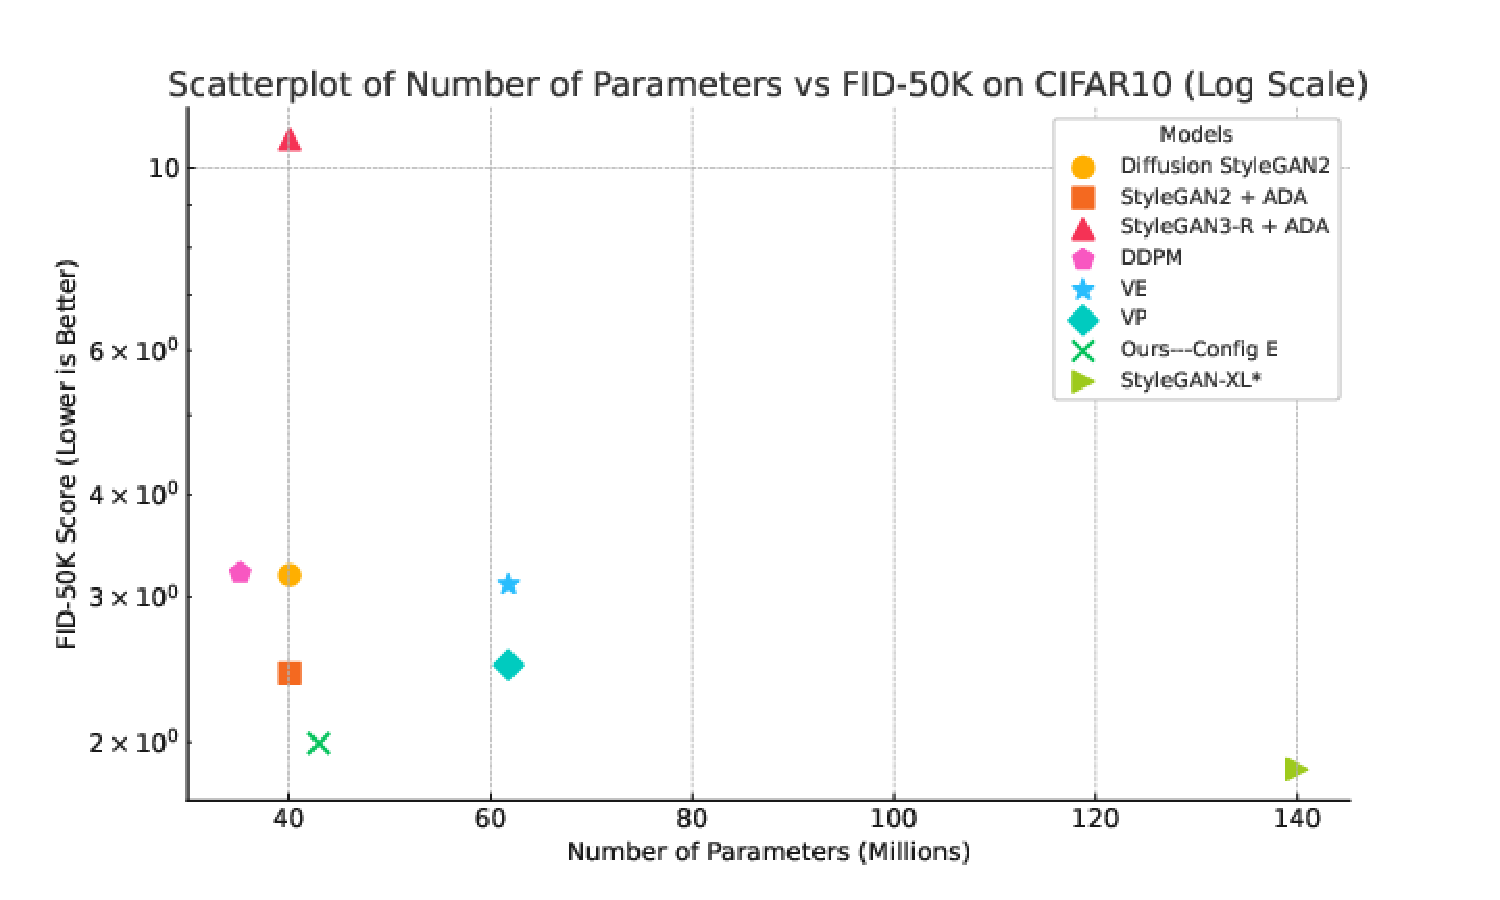
\includegraphics[width=\linewidth,clip,trim={0 0 0 2cm}]{figures/Scatterplot-FID-Parameters-CIFAR10.pdf}
    \caption{Millions of parameters vs.~FID-50K (log scale) on CIFAR-10. Lower is better.}
    \label{fig:fid-50k-vs-params-cifar-10}
\end{wrapfigure}

Many state-of-the-art GANs are derived from Projected GAN~\cite{sauer2021projected}, including StyleGAN-XL~\cite{sgxl} and the concurrent work of StyleSAN-XL~\cite{takida2024san}. These methods use a pre-trained ImageNet classifier in the discriminator. Prior work has shown that a pre-trained ImageNet discriminator can leak ImageNet features into the model~\cite{kynkaanniemi2022role}, causing the model to perform better when evaluating on FID since it relies on a pre-trained ImageNet classifier for the loss. But, this does not improve results in perceptual studies~\cite{kynkaanniemi2022role}. Our model produces its low FID without any ImageNet pre-training.

%\jt{Missing citations here for such methods.}


%\aaron{add NFEs}
%\jt{Which models in our evaluation use this? Any?}

%\jt{What is the second caveat?}

\subsection{FID --- ImageNet-32~\cite{chrabaszcz2017downsampled}}
\label{sec:imagenet32-fid-explain}
We train Config E model until convergence and with optimized hyperparameters and training schedule on ImageNet-32 (conditional generation). We compare against recent GAN models and recent diffusion models in Table~\ref{tab:imagenet32}.
We adjust the number of parameters in the generator of our model to match StyleGAN-XL~\cite{sgxl}'s generator (84M parameters). Specifically, we make the model significantly wider to match. Our method achieves comparable FID despite using a 60\% smaller discriminator (Tab.~\ref{tab:imagenet32}) and despite not using a pre-trained ImageNet classifier.
%, which has been shown to improve FID performance, but not improve results in perceptual studies~\cite{kynkaanniemi2022role}.

\vspace{-0.1cm}
\subsection{FID --- ImageNet-64~\cite{chrabaszcz2017downsampled}}
We evaluate our model on ImageNet-64 to test its scalability. We stack another resolution stage on our ImageNet-32 model, resulting in a generator of 104\ M parameters. This model is nearly 3$\times$ smaller than diffusion-like models~\cite{adm,edm,cm,icm} that rely on the ADM backbone, which contains about 300\ M parameters. Despite the smaller model size and that our model generates samples in one step, it outperforms larger diffusion models with many NFEs on FID (Tab.~\ref{tab:imagenet64}).

\vspace{-0.1cm}
\subsection{Recall}
We evaluate the recall~\cite{precrecall} of our model on each dataset to quantify sample diversity. In general, our model achieves a recall that is similar to or marginally worse than the diffusion model counterpart, yet superior to existing GAN models. For CIFAR-10, the recall of our model peaked at 0.57; as a point of comparison, StyleGAN-XL~\cite{sgxl} has a worse recall of 0.47 despite its lower FID. For FFHQ, we obtain a recall of 0.53 at 64$\times$64 and 0.49 at 256$\times$256, whereas StyleGAN2~\cite{sg2} achieved a recall of 0.43 on FFHQ-256. Our ImageNet-32 model achieved a recall of 0.63; comparable to ADM~\cite{adm}. Our ImageNet-64 model achieved recall 0.59. While this is slightly worse than $\approx$0.63 that many diffusion models achieve, it is better than BigGAN-deep~\cite{biggan} which achieved a recall of 0.48.

\begin{figure}
    \begin{floatrow}
        \capbtabbox{%
        \centering
        \resizebox{0.9\linewidth}{!}{
        \begin{tblr}{
          column{2} = {r},
          column{3} = {r},
          cell{8}{1} = {c=3}{},
          hline{2,7-8} = {-}{},
        }
    Model                                                       & NFE$\downarrow$  & FID$\downarrow$                        \\ 
    DDPM++~\cite{kim2021soft}                  & 1000 & 8.42                                   \\
    VDM~\cite{kingma2021variational}           & 1000 & 7.41                                   \\
    MSGAN~\cite{karnewar2020msg,ning2023input} & 1    & 12.3                                   \\
    ADM~\cite{adm}                             & 1000 & 3.60                                   \\
    DDPM-IP~\cite{ning2023input}               & 1000 & 2.87                                   \\
    Ours—Config E               & 1    & 1.27   \\
    \textit{With ImageNet feature leakage~\cite{kynkaanniemi2022role}:}    \\
    StyleGAN-XL*~\cite{sgxl}                   & 1    & 1.10                                  
    \end{tblr}
        }
    }{%
        \caption{\label{tab:imagenet32}ImageNet-32.}
        % \jt{some are conditional still}}
    }
    %
    \capbtabbox{
        \centering
        \resizebox{0.9\linewidth}{!}{
        \begin{tblr}{
          column{2} = {r},
          column{3} = {r},
          cell{1}{2} = {c},
          cell{1}{3} = {c},
          cell{12}{1} = {c=3}{},
          hline{2-3,11-12} = {-}{},
        }
        Model         & NFE$\downarrow$ & FID$\downarrow$ \\
        BigGAN-deep~\cite{biggan}\phantom{xx}   & 1               & 4.06            \\
        DDPM~\cite{ddpm}          & 250             & 11.0            \\
        DDIM~\cite{ddim}          & 50              & 13.7            \\
        ADM~\cite{adm}           & $^\S$250             & 2.91            \\
        EDM~\cite{edm}           & 79              & 2.23            \\
        CT~\cite{cm}            & 2               & 11.1            \\
        CD~\cite{cm}            & 3               & 4.32            \\
        iCT-deep~\cite{icm}      & 2               & 2.77            \\
        DMD~\cite{dmd}           & 1               & 2.62            \\
        Ours—Config E & 1               & 2.09            \\
        \emph{With ImageNet feature leakage~\cite{kynkaanniemi2022role}:}          &                 &                 \\
        StyleGAN-XL*~\cite{sgxl}   & 1               & 1.52            
        \end{tblr}
        }
    }
    {
        \caption{\label{tab:imagenet64}ImageNet-64.\hspace{-0.1cm} {\small \S:\hspace{-0.05cm}deterministic sampling.}}
    }
    \end{floatrow}
    \vspace{-0.25cm}
\end{figure}


% \begin{table}[ht]
%     \centering
%     \begin{tabular}{lcccccccc}
%         \toprule
%         \textbf{Model} & \textbf{\# Param.} & \textbf{IS $\uparrow$} & \textbf{FID $\downarrow$} & \textbf{Precision $\uparrow$} & \textbf{Recall $\uparrow$} & \textbf{Density $\uparrow$} & \textbf{Coverage $\uparrow$} & \textbf{Inf. (s)} \\
%         \midrule
%         ReACGAN + DiffAug (Ours) [10] & 9.4M & 10.15 & 2.64 & 0.75 & 0.65 & 0.98 & 0.90 & 0.009 \\
%         StyleGAN2-ADA [85] & 20.2M & 10.31 & 2.41 & 0.74 & 0.68 & 1.02 & 0.92 & 0.008 \\
%         StyleGAN2-ADA (Ours) [85] & 20.2M & \textbf{10.53} & 2.31 & 0.75 & 0.69 & 1.04 & 0.93 & 0.008 \\
%         StyleGAN2 + DiffAug + D2D-CE (Ours) [10] & 20.2M & 10.46 & 2.30 & 0.76 & 0.68 & 1.03 & 0.93 & 0.007 \\
%         DDPM [43] & 35.2M & 9.73 & 3.23 & 0.78 & 0.67 & 1.10 & 0.93 & 15.422 \\
%         DDPM++ [44] & 106.6M & 9.90 & 2.49 & 0.78 & 0.69 & 1.12 & 0.94 & 46.697 \\
%         NCSN++ [44] & 107.6M & 10.08 & 2.27 & 0.77 & 0.70 & 1.07 & 0.94 & 99.304 \\
%         LSGM [45] & - & 10.04 & 2.80 & 0.80 & 0.70 & 1.15 & 0.95 & - \\
%         LSGM-ODE [45] & - & 10.07 & \textbf{2.09} & 0.77 & 0.71 & 1.03 & 0.94 & - \\
%         CLD-SGM [47] & - & 9.88 & 2.38 & 0.78 & 0.69 & 1.12 & 0.94 & - \\
%         StyleGAN-XL~ & 18.0M & \textbf{11.03} & \textbf{1.88} & 0.77 & 0.59 & 1.08 & 0.94 & 0.010 \\
%         % BaselineGAN & %10.284011840820312
%         % 10.28
%         % & %1.9925376117527978 
%         % 1.99 & % 0.6899600028991699 
%         % 0.69 &&
%         \bottomrule
%     \end{tabular}
%     \caption{Comparison of various models on CIFAR10 dataset. TODO fix citation}
% \label{tab:cifar10_comparison}
%\end{table}

% \jt{Is the below meant to be a conclusion? Some of these statements are unfounded in the evidence we present so far.}
% \begin{enumerate}

%     \item We demonstrate the ability of our method to recover all modes of training data on Stacked Mnist~\ref{tab:stackedmnist}.
%     \item We beat all methods that do not use bCR (shown to overfit for FFHQ-256~\cite{}) and methods that do not leak imagenet features from a pretrained discriminator~\cite{kynkaanniemi2022role}. If we exclude these two categories of models, we are SOTA across all open source GANs. We also SOTA on a per parameter count basis on multiple GANs.
%     \item We demonstrate SOTA performance on CIFAR-10 image generation at our current parameter count, outperforming all previous GANs except for StyleGAN-XL derived ones with X\% percent of the parameters of these methods. We also do not leak features from ImageNet or use a pretrained discriminator.~\ref{tab:cifar10}. 
%     \item We achieve near SOTA on FFHQ 256 and achieve SOTA for a GAN method without bCR or feature leakage.
%     \item We achieve near state of the art results on Imagenet and achieve Pareto frontier results for total GAN model parameter size.
% \end{enumerate}
% \begin{table}[h]
\centering
\caption{FID on ImageNet-32}
\begin{tabular}{ l c c }
\toprule
Model & \textbf{Year} & FID$\downarrow$ \\
\midrule
% %Real NVP (Dinh et al.) & 2016 & 4.28 \\
% %Glow (Kingma and Dhariwal) & 2018 & 4.09 \\
% %MintNet & 2019 & 4.06 \\
% % Residual Flow & 2019 & 4.01 \\
% % BIVA Maaloe et al. & 2019 & 3.96 \\
% % ANF Huang et al. & 2020 & 3.92 \\
% % NVAE w/ flow & 2020 & 3.92 \\
% % PixelRNN & 2016 & 3.86 \\
% % Flow++ & 2019 & 3.86 \\
% % SPN Menick and Kalchbrenner & 2018 & 3.85 \\
% % Gated PixelCNN & 2016 & 3.83 \\
% % Very Deep VAE & 2020 & 3.8 \\
% % MRCNF & 2021 & 3.77 \\
% % $\delta$-VAE & 2019 & 3.77 \\
% Image Transformer~\cite{parmar2018image} & 2018 & 3.77 \\
% ScoreFlow & 2021 & 3.76 \\
% Reflected Diffusion & 2023 & 3.74 \\
% %Hourglass & 2021 & 3.74 \\
% DenseFlow-74-10 & 2021 & 3.63 \\
% i-DODE & 2023 & 3.43 \\
% MSGAN~\cite{karnewar2020msg} & 2019 & 12.3 \\
% DDPM-IP & 2023 & 2.66 \\
MSGAN~\cite{karnewar2020msg} & 2019 & 12.3 \\
VDM~\cite{kingma2021variational} & 2021 & 7.41 \\
DDPM++~\cite{kim2021soft} & 2021 & 8.42 \\
DDPM-IP~\cite{ning2023input} & 2023 & 2.87 \\
\textbf{Ours} & 2024 & 1.28 \\
StyleGAN-XL~\cite{sauer2022stylegan} & 2022 & \textbf{1.10} \\
\bottomrule
\end{tabular}
\end{table}

% \begin{table}[tO]
%     \centering
%     \begin{tabular}{c|c|c|c}
%          & FID\_50k & Precision & Recall \\
%         StyleGAN &  \\
%         StyleGAN-XL? &
%         Lots of other baselines
%     \end{tabular}
%     \caption{Caption}
%     \label{tab:my_label}
% \end{table}
% \label{sec:exp}
% % cifar10, ffhq, imagenet

% \begin{table}
%     \centering
%     %\caption{Results for CIFAR-10 generation. \aaron{add NFEs}}
%     %\vspace{-2mm}
%     \begin{tblr}{
%       column{2} = {r},
%       cell{1}{2} = {c},
%       hline{2,9,13} = {-}{},
%     }
%     Model               & FID$\downarrow$           \\
%     BigGAN~\cite{biggan}              & 14.73         \\
%     TransGAN~\cite{trans}            & 9.26          \\
%     ViTGAN~\cite{vitgan}              & 6.66          \\
%     DDGAN~\cite{ddgan}               & 3.75          \\
%     Diffusion StyleGAN2 & 3.19          \\
%     StyleGAN2 + ADA     & 2.42          \\
%     StyleGAN3-R + ADA   & 10.83         \\
%     DDPM                & 3.21          \\
%     DDIM                & 4.67          \\
%     VE                  & 3.11          \\
%     VP                  & 2.48          \\
%     Ours---Config E     & \textbf{1.99} 
%     \end{tblr}
%     %\label{tab:cifar10}
%     \caption{Results for CIFAR-10 generation. \aaron{add NFEs}}
%     \label{tab:cifar10}
% \end{table}



%%%%%%%%%%%%%%%%%%%%%%%%%%%%%%%%%%%%%%%%%%%%%%%%%%%%%%%%%%%%%
% Qualitative figures
%%%%%%%%%%%%%%%%%%%%%%%%%%%%%%%%%%%%%%%%%%%%%%%%%%%%%%%%%%%%%

% Variable to control the size of each image
% \begin{figure}
%     \centering
%     \includegraphics{example-image-a}
%     \caption{stacked mnist (qualitative figure) (from powerpoint)}
%     \label{fig:stacked-mnist}
% \end{figure}
% cifar10, ffhq, imagenet

% \noindent\begin{minipage}{.33\textwidth}
% \centering
% \captionof{table}{1000-mode coverage on StackedMNIST.}
% \vspace{-2mm}
% \begin{tblr}{
%   cell{2}{2} = {c},
%   cell{2}{3} = {c},
%   cell{3}{2} = {c},
%   cell{3}{3} = {c},
%   cell{4}{2} = {c},
%   cell{4}{3} = {c},
%   cell{5}{2} = {c},
%   cell{5}{3} = {c},
%   cell{6}{2} = {c},
%   cell{6}{3} = {c},
%   cell{7}{2} = {c},
%   cell{7}{3} = {c},
%   cell{8}{2} = {c},
%   cell{8}{3} = {c},
%   cell{9}{2} = {c},
%   cell{9}{3} = {c},
%   cell{10}{2} = {c},
%   cell{10}{3} = {c},
%   cell{11}{2} = {c},
%   cell{11}{3} = {c},
%   hline{2,11} = {1-3}{},
% }
% Model     & Modes$\uparrow$ & KLD$\downarrow$            &  \\
% DCGAN     & 99            & 3.40\phantom{0}&  \\f
% VEEGAN    & 150           & 2.95\phantom{0}&  \\
% WGAN-GP   & 959           & 0.73\phantom{0}&  \\
% PacGAN    & 992           & 0.28\phantom{0}&  \\
% StyleGAN2 & 940           & 0.42\phantom{0}&  \\
% PresGAN   & \textbf{1000} & 0.12\phantom{0}&  \\
% Adv. DSM  & \textbf{1000} & 1.49\phantom{0}&  \\
% VAEBM     & \textbf{1000} & 0.087          &  \\
% DDGAN     & \textbf{1000} & 0.071          &  \\
% Ours      & \textbf{1000} & \textbf{???} &  
% \end{tblr}
% \label{tab:stackedmnist}
% \end{minipage}%
% \begin{minipage}{.33\textwidth}
% \centering
% \captionof{table}{Results for CIFAR-10 generation.}
% \vspace{-2mm}
% \begin{tblr}{
%   column{2} = {r},
%   cell{1}{2} = {c},
%   hline{2,9,13} = {-}{},
% }
% Model               & FID$\downarrow$           \\
% BigGAN              & 14.73         \\
% TransGAN            & 9.26          \\
% ViTGAN              & 6.66          \\
% DDGAN               & 3.75          \\
% Diffusion StyleGAN2 & 3.19          \\
% StyleGAN2 + ADA     & 2.42          \\
% StyleGAN3-R + ADA   & 10.83         \\
% DDPM                & 3.21          \\
% DDIM                & 4.67          \\
% VE                  & 3.11          \\
% VP                  & 2.48          \\
% Ours                & \textbf{1.99} 
% \end{tblr}
% \label{tab:cifar10}
% \end{minipage}%
% \begin{minipage}{.33\textwidth}
% \centering
% \captionof{table}{Results on FFHQ ($256\times256$).}
% \vspace{-2mm}
% \begin{tblr}{
%   column{2} = {r},
%   cell{1}{2} = {c},
%   hline{2,5} = {-}{},
%   hline{2,9} = {-}{},
% }
% Model       & FID$\downarrow$  \\
% StyleGAN2   & 3.78 \\
% StyleGAN3-T & 4.81 \\
% StyleGAN3-R & 3.92 \\
% LDM & 4.98\\
% ADM (DDIM) & 8.41\\
% ADM (DPM-Solver) & 8.40\\
% Diffusion Autoencoder & 5.81\\
% Ours        & \textbf{2.95} 
% \end{tblr}
% \label{tab:ffhq256}
% \end{minipage}


% \input{tables/cifar10}
% \input{tables/ffhq256}
% \input{tables/MNIST}
\begin{figure}[h!]
    \newlength{\imgsize}
    \setlength{\imgsize}{0.10\linewidth} % Adjust this value to change the size of the images
    
    % New command to include images from a specific directory
    \newcommand{\qualitativeimg}[1]{%
        \includegraphics[width=\imgsize]{figures/qualitative/ffhq-256-000139623/image-#1.jpg}%
    }
    
    \setlength{\tabcolsep}{0pt} % Remove spacing between columns
    \renewcommand{\arraystretch}{0} % Remove spacing between rows
    
    \centering
    \begin{tabular}{cccccccc} % Eight columns
        \qualitativeimg{64} & \qualitativeimg{65} & \qualitativeimg{66} & \qualitativeimg{67} & \qualitativeimg{128} & \qualitativeimg{69} & \qualitativeimg{70} & \qualitativeimg{71} \\
        \qualitativeimg{72} & \qualitativeimg{73} & \qualitativeimg{74} & \qualitativeimg{75} & \qualitativeimg{76} & \qualitativeimg{77} & \qualitativeimg{78} & \qualitativeimg{79} \\
        \qualitativeimg{80} & \qualitativeimg{81} & \qualitativeimg{82} & \qualitativeimg{83} & \qualitativeimg{84} & \qualitativeimg{85} & \qualitativeimg{86} & \qualitativeimg{87} \\
        \qualitativeimg{88} & \qualitativeimg{89} & \qualitativeimg{90} & \qualitativeimg{91} & \qualitativeimg{92} & \qualitativeimg{93} & \qualitativeimg{94} & \qualitativeimg{95} \\
        \qualitativeimg{96} & \qualitativeimg{97} & \qualitativeimg{98} & \qualitativeimg{99} & \qualitativeimg{100} & \qualitativeimg{101} & \qualitativeimg{102} & \qualitativeimg{103} \\
        \qualitativeimg{104} & \qualitativeimg{105} & \qualitativeimg{106} & \qualitativeimg{107} & \qualitativeimg{108} & \qualitativeimg{109} & \qualitativeimg{110} & \qualitativeimg{111} \\
        \qualitativeimg{112} & \qualitativeimg{113} & \qualitativeimg{114} & \qualitativeimg{115} & \qualitativeimg{116} & \qualitativeimg{117} & \qualitativeimg{118} & \qualitativeimg{119} \\
        \qualitativeimg{120} & \qualitativeimg{121} & \qualitativeimg{122} & \qualitativeimg{123} & \qualitativeimg{124} & \qualitativeimg{125} & \qualitativeimg{126} & \qualitativeimg{127} \\
    \end{tabular}
    \caption{Qualitative examples of sample generation from our Config E on FFHQ-256.}
    \label{fig:ffhq-256-teaser}
\end{figure}


\section*{Acknowledgements}
This work was supported by the ERC grant number 714381 (SOLARIS project) and by the MSR-Inria joint centre.

\bibliography{bibli}
\bibliographystyle{icml2019}

\newpage

\appendix
\onecolumn


Section~\ref{sec:experiments_appx} of this supplementary presents extended results
from our experiments, along with statistical tests for assessing the significance of our findings.
Section~\ref{sec:deformation_penalties} details our lower bound penalties based on deformations
and their relationship to tangent propagation.
Section~\ref{sec:spectral_norms_appx} presents our continuation algorithm for optimization
with spectral norm constraints.
Section~\ref{sec:non_euclidian_appx} describes
heuristic extensions of our lower bound regularization strategies to non-Euclidian geometries.
Finally, Section~\ref{sec:generalization_appx} provides our proof of the margin bound
of Proposition~\ref{prop:robust_margin_bound} for adversarial generalization.

\section{Additional Experiment Results}
\label{sec:experiments_appx}

\subsection{CIFAR10}
\label{sub:cifar_appx}

This section provides more extensive results for the experiments on CIFAR10 from Section~\ref{sub:exp_smalldata}.
In particular, Table~\ref{tab:smalldata_ext} shows additional experiments on larger subsets of size 5\.000,
as well as more methods, including different geometries (see Appendix~\ref{sec:non_euclidian_appx}).
The table also reports results obtained when using a smaller validation set of size 1\,000.
The full hyper-parameter grid is given in Table~\ref{tab:smalldata_param_grid}.

In order to assess the statistical significance of our results,
we repeated the experiments on 10 new random choices of subsets, using the hyperparameters selected
on the original subset from Table~\ref{tab:smalldata_ext} (except for learning rate, which is selected according to a different validation set for each subset).
We then compared pairs of methods using a paired t-test, with p-values shown in Table~\ref{tab:t_test}.
In particular, the results strengthen some of our findings, for instance, that $\|\nabla f \|^2$
should be preferred to the gradient penalty on the loss when there is no data augmentation,
and that combined upper+lower bound approaches tend to outperform the individual upper or lower
bound strategies.


\begin{table}[h]
\caption{Regularization on CIFAR10 with 1\,000 or 5\,000 examples for VGG-11 and ResNet-18.
Extended version of Table~\ref{tab:smalldata}.
Each entry shows the test accuracy with/without data augmentation when all hyper-parameters are optimized on a validation set of size 10\,000 (a) or 1\,000 (b),
and for the epoch with highest validation accuracy,
evaluating every 10 epochs (similar to early stopping).}
\centering
\vspace{0.2cm}
\label{tab:smalldata_ext}
(a) 10k examples in validation set

% python print_table.py --full
\begin{tabular}{ | l | c | c | c | c |  }
\hline
Method & 1k VGG-11 & 1k ResNet-18 & 5k VGG-11 & 5k ResNet-18 \\ \hline
\hline
No weight decay & 50.70 / 43.75 & 45.23 / 37.12 & 72.49 / 58.35 & 72.72 / 54.12 \\
Weight decay & 51.32 / 43.95 & 44.85 / 37.09 & 72.80 / 58.56 & 73.06 / 53.33 \\
SN penalty (PI) & 54.64 / 45.06 & 47.01 / 39.63 & 74.03 / 62.45 & 74.79 / 54.04 \\
SN penalty (SVD) & 53.44 / 46.06 & 47.26 / 37.94 & 74.53 / 62.93 & 75.59 / 54.98 \\
SN projection & 54.14 / \textbf{\color{darkgray}46.70} & 47.12 / 37.28 & 75.14 / 63.81 & 76.23 / 55.60 \\
VAT & 50.88 / 43.36 & 47.47 / 42.82 & 72.91 / 58.78 & 71.56 / 55.93 \\
PGD-$\ell_2$ & 51.25 / 44.40 & 45.80 / 41.87 & 73.18 / 58.98 & 72.53 / 55.92 \\
PGD-$\ell_\infty$ & 51.17 / 43.07 & 45.31 / 39.66 & 73.05 / 57.82 & 72.75 / 55.14 \\
grad-$\ell_2$ & \textbf{\color{darkgray}55.19} / 43.88 & \textbf{49.30} / \textbf{\color{darkgray}44.65} & \textbf{75.38} / 59.20 & 75.22 / 55.36 \\
grad-$\ell_1$ & 54.88 / 44.74 & \textbf{\color{darkgray}49.06} / 42.63 & \textbf{\color{darkgray}75.25} / 59.39 & 74.48 / 56.19 \\
\hline
$\|f\|_\delta^2$ penalty & 51.41 / 45.07 & 48.73 / 43.72 & 72.98 / 61.45 & 72.78 / 56.50 \\
$\|\nabla f\|^2$ penalty & 54.80 / 46.37 & \textbf{\color{darkgray}48.99} / \textbf{44.97} & 73.90 / 60.17 & 73.83 / \textbf{\color{darkgray}57.92} \\
PGD-$\ell_2$ + SN proj & 54.19 / \textbf{\color{darkgray}46.66} & 47.47 / 41.25 & 74.61 / \textbf{64.50} & \textbf{\color{darkgray}77.19} / 57.43 \\
grad-$\ell_2$ + SN proj & \textbf{55.32} / \textbf{46.88} & 48.73 / 42.78 & 75.11 / 63.54 & \textbf{77.73} / 57.09 \\
$\|f\|_\delta^2$ + SN proj & 54.02 / \textbf{\color{darkgray}46.72} & 48.12 / 43.56 & 74.55 / \textbf{\color{darkgray}64.33} & 75.64 / \textbf{59.03} \\
$\|\nabla f\|^2$ + SN proj & \textbf{55.24} / \textbf{46.80} & \textbf{\color{darkgray}49.06} / \textbf{44.92} & 72.31 / 63.74 & 72.24 / 57.56 \\
\hline
\end{tabular}
\\
\vspace{0.2cm}
(b) 1k examples in validation set

% python print_table.py --full --small_val
\begin{tabular}{ | l | c | c | c | c |  }
\hline
Method & 1k VGG-11 & 1k ResNet-18 & 5k VGG-11 & 5k ResNet-18 \\ \hline
\hline
No weight decay & 51.32 / 43.42 & 45.00 / 37.00 & 72.64 / 57.88 & 72.71 / 53.80 \\
Weight decay & 51.04 / 43.42 & 44.66 / 36.77 & 72.68 / 57.59 & 72.25 / 54.16 \\
SN penalty (PI) & 54.60 / 44.20 & 46.39 / 38.86 & 72.99 / 62.49 & 74.72 / 53.65 \\
SN penalty (SVD) & 53.76 / 44.79 & 47.31 / 37.92 & 74.05 / 63.34 & 75.73 / 54.65 \\
SN projection & 52.86 / \textbf{\color{darkgray}46.49} & 47.05 / 37.28 & 74.18 / \textbf{\color{darkgray}63.70} & 75.91 / 54.43 \\
VAT & 50.90 / 43.99 & 47.35 / 42.91 & 72.95 / 57.64 & 71.91 / 55.22 \\
PGD-$\ell_2$ & 50.95 / 43.26 & 45.77 / 41.71 & 72.71 / 57.68 & 72.87 / 54.17 \\
PGD-$\ell_\infty$ & 51.16 / 43.16 & 45.67 / 39.77 & 73.64 / 58.02 & 72.99 / 53.95 \\
grad-$\ell_2$ & \textbf{55.40} / 43.57 & 47.86 / \textbf{\color{darkgray}44.65} & \textbf{75.44} / 58.33 & 74.83 / 55.43 \\
grad-$\ell_1$ & 54.53 / 43.04 & \textbf{\color{darkgray}48.75} / 42.21 & \textbf{\color{darkgray}75.28} / 58.19 & 74.28 / 54.02 \\
\hline
$\|f\|_M^2$ penalty & 51.00 / 44.67 & 48.57 / 44.30 & 72.76 / 60.55 & 72.75 / 56.49 \\
$\|\nabla f\|^2$ penalty & 54.68 / 46.10 & 48.53 / \textbf{45.21} & 73.83 / 60.36 & 73.30 / \textbf{\color{darkgray}57.46} \\
PGD-$\ell_2$ + SN proj & 53.85 / \textbf{46.79} & 46.48 / 40.95 & 74.79 / 63.37 & \textbf{\color{darkgray}76.28} / \textbf{\color{darkgray}57.43} \\
grad-$\ell_2$ + SN proj & \textbf{\color{darkgray}55.28} / 45.11 & 48.42 / 41.93 & 75.17 / 63.45 & \textbf{77.24} / 56.18 \\
$\|f\|_M^2$ + SN proj & 54.00 / 45.14 & 47.12 / 41.86 & 74.54 / \textbf{63.94} & 75.25 / \textbf{57.94} \\
$\|\nabla f\|^2$ + SN proj & \textbf{\color{darkgray}55.21} / 45.68 & \textbf{49.03} / 43.58 & 71.92 / 63.47 & 71.83 / 56.06 \\
\hline
\end{tabular}
\end{table}


\begin{table}[h]
\caption{Paired t-tests comparing pairs of methods, on 10 different random choices of subsets of CIFAR10.
Each cell shows the p-value of the corresponding test, both with (left) and without (right) data augmentation.
We only show p-values smaller than~$0.05$.
Hyperparameters are fixed to the ones obtained for the results in Table~\ref{tab:smalldata}
(selected on a different choice of subset), except for the learning rate which is tuned on
a separate validation set for each choice of subset.}
\centering
\label{tab:t_test}
\vspace{0.2cm}
% python print_significance_table.py --test_type ttest --optlr
\begin{tabular}{ | c | c c | c c | c c | c c |  }
\hline
Test & \multicolumn{2}{|c|}{1k VGG-11} & \multicolumn{2}{|c|}{1k ResNet-18} & \multicolumn{2}{|c|}{5k VGG-11} & \multicolumn{2}{|c|}{5k ResNet-18} \\ \hline
\hline
SN projection $\succ$ Weight decay & 1e-04 & 1e-03 & - & - & 3e-06 & 1e-08 & 9e-07 & 4e-04\\ \hline
grad-$\ell_2$ $\succ$ Weight decay & 4e-09 & - & 2e-04 & 5e-05 & 7e-08 & 1e-04 & 5e-06 & -\\ \hline
$\|\nabla f\|^2$ $\succ$ Weight decay & 1e-08 & 2e-07 & 1e-05 & 3e-07 & 3e-04 & 5e-07 & 7e-03 & 1e-06\\ \hline
$\|\nabla f\|^2$ $\succ$ grad-$\ell_2$ & - & 3e-08 & 2e-02 & 2e-06 & - & 6e-05 & - & 4e-05\\ \hline
grad-$\ell_2$ $\succ$ $\|\nabla f\|^2$ & 2e-02 & - & - & - & 2e-05 & - & 7e-04 & -\\ \hline
grad-$\ell_2$ + SN proj $\succ$ grad-$\ell_2$ & - & 9e-03 & - & - & - & 5e-07 & 9e-06 & 2e-04\\ \hline
$\|\nabla f\|^2$ + SN proj $\succ$ $\|\nabla f\|^2$ & - & - & - & 1e-02 & - & 2e-06 & - & -\\ \hline
\end{tabular}
\end{table}

\begin{table}[h]
\caption{List of hyper-parameters used for each method on CIFAR10.
For each method, we additionally consider a learning rate parameter in $[0.003 ; 0.01 ; 0.03 ; 0.1]$.
For combined penalties, the sets of hyperparameters are listed in the same order as in the first column
(\ie, the choices of constraint radius are given last).}
\centering
\small
\vspace{0.2cm}
\label{tab:smalldata_param_grid}
\begin{tabular}{ | l | c |  }
\hline
Method & Parameter grid \\ \hline
\hline
No weight decay &  -   \\ \hline
Weight decay &  $[0; 0.0001 ; 0.0002 ; 0.0004 ; 0.0008 ; 0.001 ; 0.002]$   \\ \hline
SN penalty (PI) &  $[0.001 ; 0.003 ; 0.01 ; 0.03 ; 0.1 ; 0.3]$ \\ \hline
SN penalty (SVD) &  $[0.001 ; 0.003 ; 0.01 ; 0.03 ; 0.1 ; 0.3]$  \\ \hline
SN projection &  $[0.5 ; 0.6 ; 0.8 ; 1.0 ; 1.2 ; 1.4]$  \\ \hline
$\|f\|_\delta^2$ penalty & $[0.001 ; 0.003 ; 0.01 ; 0.03 ; 0.1]$  \\ \hline
$\|\nabla f\|^2$ penalty & $[0.00003 ; 0.0001 ; 0.0003 ; 0.001 ; 0.003 ; 0.01 ; 0.03]$ \\ \hline
VAT & $[0.1 ; 0.3 ; 1.0 ; 3.0]$ \\ \hline
PGD-$\ell_2$ &  $[0.003 ; 0.01 ; 0.03 ; 0.1 ; 0.3 ; 1.0]$ \\ \hline
PGD-$\ell_\infty$ &  $[0.001 ; 0.003 ; 0.01 ; 0.03 ; 0.1 ; 0.3]$  \\ \hline
grad-$\ell_1$ &  $[0.0001 ; 0.0003 ; 0.001 ; 0.003 ; 0.01 ; 0.03]$  \\ \hline
grad-$\ell_2$ &  $[0.001 ; 0.003 ; 0.01 ; 0.03 ; 0.1 ; 0.3 ; 1.0 ; 3.0]$ \\ \hline
PGD-$\ell_2$ + SN projection &  $ [0.003 ; 0.01 ; 0.03 ; 0.1] \times [0.6 ; 1.0 ; 1.4]$   \\ \hline
grad-$\ell_2$ + SN projection & $ [0.003 ; 0.01 ; 0.03 ; 0.1] \times [0.6 ; 1.0 ; 1.4]$  \\ \hline
$\|f\|_\delta^2$ + SN projection & $ [0.003 ; 0.01 ; 0.03] \times [0.6 ; 1.0 ; 1.4]$    \\ \hline
$\|\nabla f\|^2$ + SN projection & $ [0.001 ; 0.01 ; 0.1] \times [0.6 ; 1.0 ; 1.4]$   \\ \hline
\end{tabular}
\end{table}

\subsection{Infinite MNIST}
\label{sub:imnist_appx}

We provide more extensive results for the Infinite MNIST dataset in Table~\ref{tab:imnist_ext},
in particular showing more regularization strategies, as well as results with or without
data augmentation, marked with~$(\ast)$.
As in the case of CIFAR10, we use SGD with momentum (fixed to 0.9) for 500 epochs,
with initial learning rates in~$[0.005; 0.05; 0.5]$, and divide the step-size by 2 every 40 epochs.
The full hyper-parameter grid is given in Table~\ref{tab:imnist_param_grid}.


As in the case of CIFAR10, we report statistical significance tests in Table~\ref{tab:imnist_ttests} comparing pairs of
methods based on 10 different random choices of subsets.
In particular, the results confirm that weight decay with data augmentation alone
tends to give weaker results than separate penalties,
and that the combined penalty $\|f\|_\tau^2 + \|f\|_\delta^2$, which combines adversarial
perturbations of two different types,
outperforms each penalty taken by itself on a single type of perturbation,
which emphasizes the benefit of considering perturbations of different natures,
perhaps thanks to a tighter lower bound approximation of the RKHS norm.
We note that grad-$\ell_2 (\ast)$ worked well on some subsets,
but poorly on others due to training instabilities,
possibly because of the selected hyperparameters which are quite large
(and thus likely violate the approximation to the robust optimization objective).

\begin{table}
\caption{Test accuracies on subsets of MNIST using deformations from Infinite MNIST.
Extended version of Table~\ref{tab:imnist}.
($\ast$) indicates that random deformations were included as training examples (\ie, data augmentation),
while $\|f\|_\tau^2$ and $\|D_\tau f\|^2$
use them as part of the regularization penalty.
As in Table~\ref{tab:smalldata_ext}, we show results obtained using a validation set
of size 10\,000 (a) and 1\,000 (b).
}
\centering
\vspace{0.2cm}
\label{tab:imnist_ext}
\begin{tabular}{c c}
(a) 10k examples in validation set
& (b) 1k examples in validation set \\

% python print_table_imnist.py --lr --appendix
\begin{tabular}{ | l | c | c |  }
\hline
Method & 300 VGG & 1k VGG \\ \hline
\hline
Weight decay & 89.32 & 94.08 \\
Weight decay ($\ast$) & 92.41 & 95.64 \\
SN projection & 90.69 & 95.01 \\
SN projection ($\ast$) & 92.17 & 95.88 \\
grad-$\ell_2$ & 93.63 & 96.67 \\
grad-$\ell_2$ ($\ast$) & 95.05 & 97.48 \\
\hline
$\|f\|_\delta^2$ penalty & 94.17 & 96.99 \\
$\|f\|_\delta^2$ penalty ($\ast$) & 94.86 & 97.40 \\
$\|\nabla f\|^2$ penalty & 94.08 & 96.82 \\
$\|\nabla f\|^2$ penalty ($\ast$) & 94.80 & 97.29 \\
$\|D_\tau f\|^2$ penalty & 94.18 & 96.98 \\
$\|D_\tau f\|^2$ penalty ($\ast$) & 94.91 & 97.29 \\
$\|f\|_\tau^2$ penalty & 94.42 & 97.13 \\
$\|f\|_\tau^2$ penalty ($\ast$) & 94.83 & 97.25 \\
$\|f\|_{\tau}^2$ + $\|\nabla f\|^2$ & 94.75 & 97.40 \\
$\|f\|_{\tau}^2$ + $\|\nabla f\|^2$ ($\ast$) & 95.14 & 97.44 \\
$\|f\|_{\tau}^2$ + $\|f\|^2_\delta$ & 95.23 & \textbf{\color{darkgray}97.66} \\
$\|f\|_{\tau}^2$ + $\|f\|^2_\delta$ ($\ast$) & \textbf{95.53} & \textbf{\color{darkgray}97.56} \\
grad-$\ell_2$ + SN proj & 93.89 & 96.85 \\
grad-$\ell_2$ + SN proj ($\ast$) & 95.15 & \textbf{97.80} \\
$\|f\|_\delta^2$ + SN proj & 93.97 & 96.89 \\
$\|f\|_\delta^2$ + SN proj ($\ast$) & 94.78 & 97.38 \\
$\|f\|_{\tau}^2$ + $\|\nabla f\|^2$ + SN proj & 95.09 & 97.42 \\
$\|f\|_{\tau}^2$ + $\|\nabla f\|^2$ + SN proj ($\ast$) & 95.03 & 97.27 \\
$\|f\|_{\tau}^2$ + $\|f\|^2_\delta$ + SN proj & 95.20 & \textbf{\color{darkgray}97.60} \\
$\|f\|_{\tau}^2$ + $\|f\|^2_\delta$ + SN proj ($\ast$) & \textbf{\color{darkgray}95.40} & \textbf{97.77} \\
\hline
\end{tabular}
&
% python print_table_imnist.py --lr --appendix --small_val
\begin{tabular}{ | l | c | c |  }
\hline
Method & 300 VGG & 1k VGG \\ \hline
\hline
Weight decay & 89.32 & 93.34 \\
Weight decay ($\ast$) & 91.91 & 95.73 \\
SN projection & 90.60 & 94.83 \\
SN projection ($\ast$) & 92.01 & 95.91 \\
grad-$\ell_2$ & 92.92 & 96.42 \\
grad-$\ell_2$ ($\ast$) & \textbf{\color{darkgray}94.69} & \textbf{\color{darkgray}97.48} \\
\hline
$\|f\|_M^2$ penalty & 93.44 & 96.98 \\
$\|f\|_M^2$ penalty ($\ast$) & 94.57 & 97.14 \\
$\|\nabla f\|^2$ penalty & 94.08 & 96.77 \\
$\|\nabla f\|^2$ penalty ($\ast$) & 94.50 & 97.15 \\
$\|D_\tau f\|^2$ penalty & 94.03 & 97.16 \\
$\|D_\tau f\|^2$ penalty ($\ast$) & 94.15 & 96.64 \\
$\|f\|_\tau^2$ penalty & 93.53 & 97.13 \\
$\|f\|_\tau^2$ penalty ($\ast$) & \textbf{\color{darkgray}94.79} & 97.26 \\
$\|f\|_{\tau}^2$ + $\|\nabla f\|^2$ & \textbf{\color{darkgray}94.75} & 97.21 \\
$\|f\|_{\tau}^2$ + $\|\nabla f\|^2$ ($\ast$) & 94.43 & \textbf{\color{darkgray}97.42} \\
$\|f\|_{\tau}^2$ + $\|f\|^2_M$ & \textbf{95.15} & 97.27 \\
$\|f\|_{\tau}^2$ + $\|f\|^2_M$ ($\ast$) & \textbf{95.20} & \textbf{\color{darkgray}97.49} \\
grad-$\ell_2$ + SN proj & 93.44 & 96.81 \\
grad-$\ell_2$ + SN proj ($\ast$) & 94.05 & \textbf{97.60} \\
$\|f\|_M^2$ + SN proj & 93.97 & 96.61 \\
$\|f\|_M^2$ + SN proj ($\ast$) & \textbf{\color{darkgray}94.69} & 97.33 \\
$\|f\|_{\tau}^2$ + $\|\nabla f\|^2$ + SN proj & \textbf{\color{darkgray}94.75} & 97.16 \\
$\|f\|_{\tau}^2$ + $\|\nabla f\|^2$ + SN proj ($\ast$) & \textbf{\color{darkgray}94.74} & 97.22 \\
$\|f\|_{\tau}^2$ + $\|f\|^2_M$ + SN proj & \textbf{\color{darkgray}94.78} & \textbf{\color{darkgray}97.49} \\
$\|f\|_{\tau}^2$ + $\|f\|^2_M$ + SN proj ($\ast$) & \textbf{95.17} & \textbf{97.64} \\
\hline
\end{tabular}
\end{tabular}
\end{table}

\begin{table}
\caption{Paired t-tests comparing pairs of methods,
on 10 different random choices of subsets of MNIST.
Each cell shows the p-value of the corresponding test.
We only show p-values smaller than~$0.05$.
Hyperparameters are fixed to the ones obtained for the results in Table~\ref{tab:imnist}
(selected on a different choice of subset), except for the learning rate which is tuned on
a separate validation set for each choice of subset.
}
\centering
\vspace{0.2cm}
\label{tab:imnist_ttests}
% python print_significance_table_imnist.py --test_type ttest --optlr
\begin{tabular}{ | c | c | c |  }
\hline
Test & 300 VGG & 1k VGG \\ \hline
\hline
grad-$\ell_2$ ($\ast$) $\succ$ Weight decay ($\ast$) & - & 3e-11\\ \hline
$\|f\|_\tau^2$ penalty $\succ$ Weight decay ($\ast$) & 2e-08 & 2e-10\\ \hline
$\|f\|_{\tau}^2$ + $\|f\|^2_\delta$ $\succ$ Weight decay ($\ast$) & 1e-08 & 2e-10\\ \hline
$\|f\|_{\tau}^2$ + $\|f\|^2_\delta$ + SN proj ($\ast$) $\succ$ grad-$\ell_2$ ($\ast$) & - & 1e-02\\ \hline
grad-$\ell_2$ ($\ast$) $\succ$ $\|f\|_{\tau}^2$ + $\|f\|^2_\delta$ + SN proj ($\ast$) & - & -\\ \hline
$\|f\|_{\tau}^2$ + $\|f\|^2_\delta$ $\succ$ $\|f\|_\delta^2$ penalty & 1e-07 & 6e-09\\ \hline
$\|f\|_{\tau}^2$ + $\|f\|^2_\delta$ $\succ$ $\|f\|_\tau^2$ penalty & 2e-06 & 6e-07\\ \hline
$\|f\|_{\tau}^2$ + $\|f\|^2_\delta$ ($\ast$) $\succ$ $\|f\|_{\tau}^2$ + $\|f\|^2_\delta$ & 2e-03 & -\\ \hline
$\|f\|_{\tau}^2$ + $\|f\|^2_\delta$ + SN proj ($\ast$) $\succ$ $\|f\|_{\tau}^2$ + $\|f\|^2_\delta$ & 2e-03 & 2e-04\\ \hline
\end{tabular}
\end{table}


\begin{table}
\caption{List of hyper-parameters used for each method on Infinite MNIST.
For each method, we additionally consider a learning rate parameter in $[0.005 ; 0.05 ; 0.5]$.
For combined penalties, the sets of hyperparameters are listed in the same order as in the first column
(\eg, the choices of constraint radius are given last).}
\centering
\small
\vspace{0.2cm}
\label{tab:imnist_param_grid}
\begin{tabular}{ | l | c | }
\hline
Method & Grid \\ \hline
\hline
Weight decay & [0; 0.00001; 0.00003; 0.0001; 0.0003; 0.001; 0.003; 0.01; 0.03; 0.1] \\
SN projection & [1.0; 1.2; 1.4; 1.6; 1.8] \\
grad-$\ell_2$ & [0.1; 0.3; 1.0; 3.0; 10.0] \\
$\|f\|_\delta^2$ penalty & [0.1; 0.3; 1.0; 3.0] \\
$\|\nabla f\|^2$ penalty & [0.0003; 0.001; 0.003; 0.01; 0.03; 0.1; 0.3] \\
$\|D_\tau f\|^2$ penalty & [0.003; 0.01; 0.03; 0.1; 0.3] \\
$\|f\|_\tau^2$ penalty & [0.03; 0.1; 0.3; 1.0; 3.0] \\
$\|f\|_{\tau}^2$ + $\|\nabla f\|^2$ & [0.03; 0.1; 0.3; 1.0] $\times$ [0.003; 0.01; 0.03; 0.1] \\
$\|f\|_{\tau}^2$ + $\|f\|^2_\delta$ & [0.1; 0.3; 1.0] $\times$ [0.03; 0.1] \\
grad-$\ell_2$ + SN proj & [0.3; 1.0; 3.0; 10.0; 30.0] $\times$ [1.2; 1.6; 2.0] \\
$\|f\|_\delta^2$ + SN proj & [0.03; 0.1] $\times$ [1.2; 1.6; 2.0] \\
$\|f\|_{\tau}^2$ + $\|\nabla f\|^2$ + SN proj & [0.03; 0.1; 0.3] $\times$ [0.01; 0.03; 0.1] $\times$ [1.2; 1.6; 2.0] \\
$\|f\|_{\tau}^2$ + $\|f\|^2_\delta$ + SN proj & [0.1; 0.3; 1.0] $\times$ [0.03; 0.1] $\times$ [1.2; 1.6; 2.0] \\
\hline
\end{tabular}
\end{table}

\subsection{Protein homology detection}
\label{sub:protein_appx}

\paragraph{Dataset description.}
Our protein homology detection experiments consider
the Structural Classification Of Proteins (SCOP) version 1.67 dataset \citep{murzin1995scop},
filtered and split following the procedures of \cite{haandstad2007motif}.
Specifically, positive training samples are extracted from one superfamily from which one family is withheld to serve as positive test set, while negative sequences are chosen from outside of the target family’s hold and are randomly split into training and test samples in the same ratio as positive samples.
This yields 102 superfamily classification tasks, which are generally very class-imbalanced.
For each task, we sample 100 class-balanced training samples to use as training set. The positive samples are extended to 50 with Uniref50 using PSI-BLAST \citep{altschul1997gapped} if they are fewer.

\paragraph{Data augmentation procedure.}
We consider in our experiments a discrete way of perturbing training samples to 
perform data augmentation. Specifically, for a given sequence, a perturbed sequence 
can be obtained by randomly changing some of the characters. Each character in the sequence 
is switched to a different one, randomly chosen from the alphabet, with some 
probability $p$. We fixed this probability to 0.1 throughout the experiments.

\paragraph{Experimental details and significance tests.}
In our experiments, we use the Adam optimization algorithm with a learning rate fixed
to 0.01 (and $\beta$ fixed to defaults $(0.9, 0.999)$),
with a batch size of 100 for 300 epochs.
The full hyper-parameter grid is given in Table~\ref{tab:protein_param_grid}.
In addition to the average auROC50 scores reported in Table~\ref{tab:protein},
we perform paired t-tests for comparing pairs of methods in Table~\ref{tab:protein_ttests}
in order to verify the significance of our findings.
The results confirm that the adversarial perturbation penalty and its combination
with spectral norm constraints tends to outperform the other approaches.


\begin{table}
\caption{Paired t-tests comparing pairs of methods on the 51 test datasets from the
set of protein homology detection tasks.
Each cell shows the p-value of the corresponding test.
We only show p-values smaller than~$0.05$.
We use the same hyperparameters as the ones obtained in the results of Table~\ref{tab:protein}.
}
\centering
\vspace{0.2cm}
\label{tab:protein_ttests}
\begin{tabular}{|l|c|c|}
\hline
 Test                                                            &   No DA &      DA \\ \hline
\hline
 SN proj $\succ$ Weight decay                                    &   1e-05 &   4e-05 \\
 grad-$\ell_2$ $\succ$ Weight decay                              &   5e-05 &   5e-02 \\
 $\|f\|_{\delta}^2$ $\succ$ Weight decay                         &   5e-06 &   3e-05 \\
 $\|\nabla f\|^2$ $\succ$ Weight decay                           &   9e-06 &   3e-03 \\
 $\|f\|_{\delta}^2$ $\succ$ grad-$\ell_2$                        &   -     &   4e-03 \\
 $\|\nabla f\|^2$ $\succ$ grad-$\ell_2$                          &   -     &   -     \\
 grad-$\ell_2$ + SN proj $\succ$ grad-$\ell_2$                   &   -     &   1e-03 \\
 $\|f\|_{\delta}^2$ + SN proj $\succ$ $\|f\|_{\delta}^2$         &   3e-03 &   5e-02 \\
 $\|\nabla f\|^2$ + SN proj $\succ$ $\|\nabla f\|^2$             &   -     &   -     \\
 $\|f\|_{\delta}^2$ + SN proj $\succ$ $\|\nabla f\|^2$ + SN proj &   8e-05 &   -     \\
\hline
\end{tabular}
\end{table}

\begin{table}
\caption{List of hyper-parameters used for each method on protein homology detection datasets.
For combined penalties, the hyperparameters are the cross-products of each individual method.}
\centering
\small
\vspace{0.2cm}
\label{tab:protein_param_grid}
\begin{tabular}{|c|c|}
\hline
 Method                                                       &   Parameter grid \\ \hline
\hline
 No weight decay  &  $-$                          \\
 Weight decay     &  $[0; 0.01; 0.001; 0.0001; 0.00001]$ \\
 SN proj          &  $[10; 1.0; 0.1]$             \\
 PGD-$\ell_2$     &  $[100.0; 10.0; 1.0; 0.1]$    \\
 grad-$\ell_2$    &  $[100.0; 10.0; 1.0; 0.1; 0.01, 0.001]$     \\
 $\|f\|_{\delta}^2$      &  $[10.0; 1.0; 0.1]$           \\
 $\|\nabla f\|^2$ &  $[10.0; 1.0; 0.1; 0.01; 0.001; 0.0001]$ \\
\hline
\end{tabular}
\end{table}


\subsection{Robustness}
\label{sub:robustness_appx}

Figure~\ref{fig:robust_tradeoffs_appx} extends Figure~\ref{fig:robust_tradeoffs}
from Section~\ref{sub:exp_robust} to show more methods, adversary strenghts, and different geometries.
For combined (PGD-$\ell_2$ + SN projection) approaches, we can see that stronger constraints (\ie, smaller~$\tau$)
tend to reduce standard accuracy, likely because it prevents a good fit of the data,
but can provide better robustness to strong adversaries ($\epsilon_{test} = 1$).
We can see that using the right metric in PGD indeed helps against an~$\ell_\infty$ adversary,
nevertheless controlling global stability through the RKHS norm as in the~$\|f\|_\delta^2$ and~$\|\nabla f\|^2$
penalties can still provide some robustness against such adversaries, even with large $\epsilon_{test}$.
For gradient penalties, we find that the different geometries behave quite similarly,
which may suggest that more appropriate optimization algorithms than SGD could be needed to
better accommodate the non-smooth case of $\ell_1/\ell_\infty$, or perhaps that both algorithms are actually
controlling the same notion of complexity on this dataset.


\begin{figure*}
	\centering
	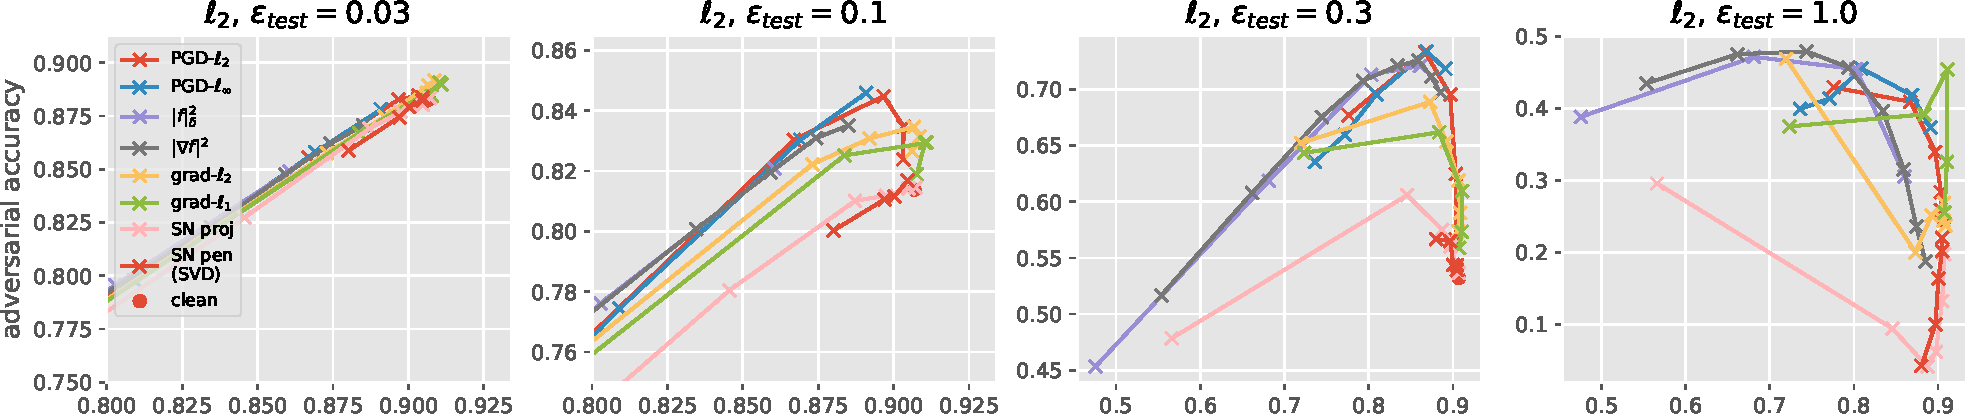
\includegraphics[width=.9\textwidth]{figures/cifar10_vgg/test_vs_adv_l2.pdf}
	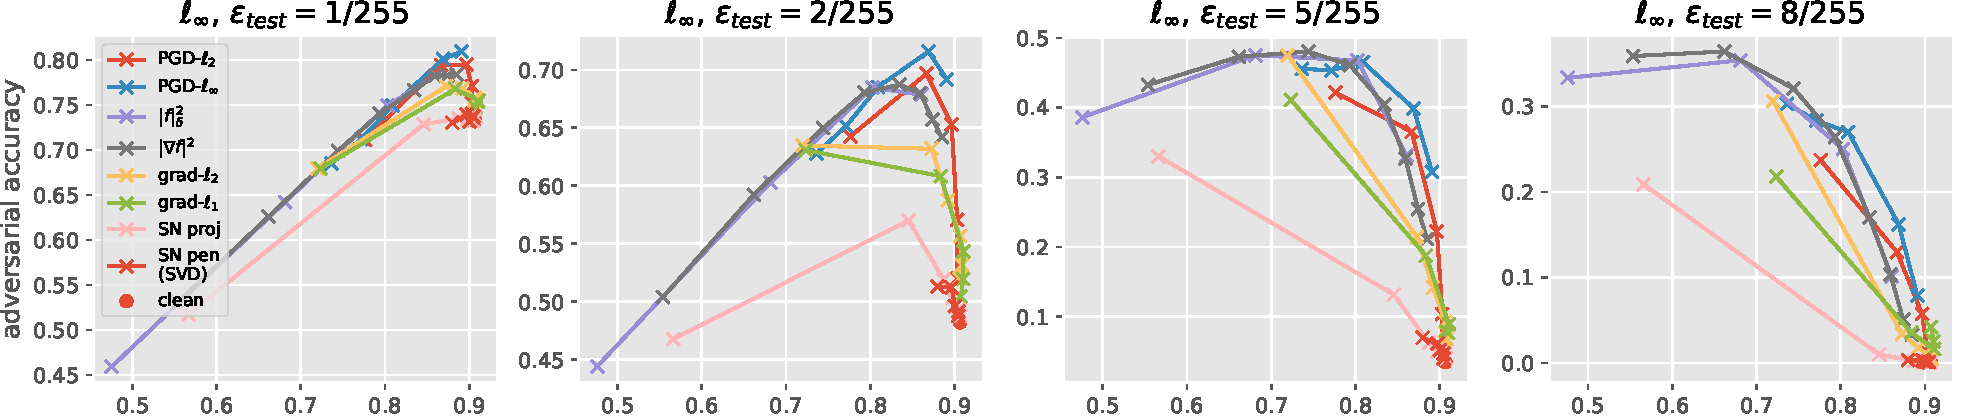
\includegraphics[width=.9\textwidth]{figures/cifar10_vgg/test_vs_adv_linf.pdf}
	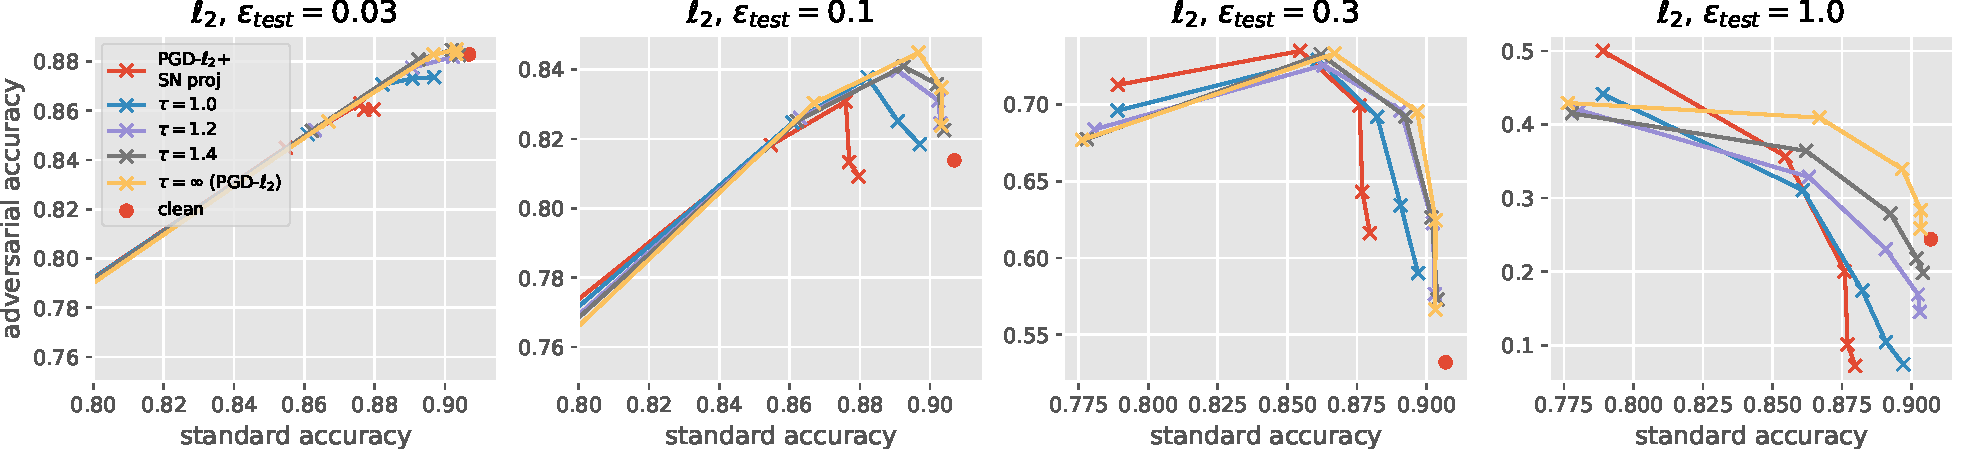
\includegraphics[width=.9\textwidth]{figures/cifar10_vgg/test_vs_adv_comb.pdf}
	\caption{Robustness trade-off curves of different regularization methods for VGG11 on CIFAR10 (extended
	version of Figure~\ref{fig:robust_tradeoffs}).
	The plots show test accuracy vs adversarial test accuracy
	for $\ell_2$-bounded (top/bottom) or $\ell_\infty$-bounded (middle),
	40-step PGD adversaries with a fixed~$\epsilon_{\text{test}}$.
	Different points on a curve correspond to training with different regularization strengths.
	The regularization increases monotonically along a given curve, and
	the leftmost points correspond to the strongest regularization.
	The bottom plots consider PGD-$\ell_2$ + SN projection,
	with different fixed values of the constraint radius~$\tau$, for varying $\epsilon$ in PGD.}
	\label{fig:robust_tradeoffs_appx}
\end{figure*}


\clearpage

\section{Details on Deformation Stability Penalties}
\label{sec:deformation_penalties}
%!TEX root = main.tex

This section provides more details on the deformation stability penalties mentioned in
Section~\ref{sub:lower_bounds}, and the practical versions we use in our experiments on the
Infinite MNIST dataset~\citep{loosli-canu-bottou-2006}.

\paragraph{Stability to deformations.}
We begin by providing some background on deformation stability,
recalling that these can provide new lower bound penalties as explained in Section~\ref{sub:lower_bounds}.
Viewing an element $x \in \mathcal X$ as a signal $x(u)$, where $u$ denotes the location
(\eg~a two-dimensional vector for images),
we denote by $x_\tau$ a deformed version of~$x$ given by $x_\tau(u) = x(u - \tau(u))$,
where~$\tau$ is a diffeomorphism.
The deformation stability bounds of~\citet{bietti2018group} take the form:
\begin{equation}
\label{eq:stability_bound}
\|\Phi(x_\tau) - \Phi(x)\|_\Hcal \leq (C_1 \|\tau\|_\infty + C_2 \|\nabla \tau\|_\infty) \|x\|,
\end{equation}
where $\nabla \tau (u)$ is the Jacobian of $\tau$ at location~$u$.
Here, $C_1$ controls translation invariance and typically decreases with the total amount of pooling
(\ie, translation invariance more or less corresponds to the resolution at the final layer),
while~$C_2$ controls stability to deformations (note that $\nabla \tau = 0$ for translations)
and is typically smaller when using small patches.
We note that the bounds assume linear pooling layers with a certain spatial decay,
adapted to the resolution of the current layer;
our experiments on Infinite MNIST with deformation stability penalties
thus use average pooling layers on 2x2 neighborhoods.


\paragraph{Adversarial deformation penalty.}
We can obtain lower bound penalties by exploiting the above stability bounds in
a similar manner to the adversarial perturbation penalty introduced in Section~\ref{sub:lower_bounds}.
In particular, assuming a scalar-valued convolutional network~$f$:
\begin{equation}
\label{eq:adv_deformation}
\|f\|_\tau^2 := \sup_{x \in \mathcal X, \tau \in \mathcal T} (f(x_\tau) - f(x))^2 \\
\end{equation}
where~$\mathcal T$ is a collection of diffeomorphisms.
When the diffeomorphisms in~$\mathcal T$ have bounded norm~$\|\tau\|_\infty$ and
Jacobian norm~$\|\nabla \tau\|_\infty$,
and assuming $\mathcal X$ (or, in practice, the training data) is bounded,
the stability bound~\ref{eq:stability_bound} ensures that
the set $U_{\mathcal T} = \{\Phi(x_\tau) - \Phi(x) : x \in \mathcal X, \tau \in \mathcal T\}$ is included in an
RKHS ball with some radius $r$, so that~$\|f\|_\tau$ is a lower bound on~$r \|f\|_\Hcal$.

\paragraph{Tangent gradient penalty.}
We also consider the following gradient penalty along tangent vectors,
which provides an approximation of the above adversarial penalty when
considering small, parameterized deformations,
and recovers the tangent propagation strategy of~\citet{simard1998transformation}:
\begin{equation}
\label{eq:tangent_gradient}
\|D_\tau f\|^2 := \sup_{x \in \mathcal X} \|\partial_\alpha f(x + \sum_i \alpha_i t_{x,i}) \|^2,
\end{equation}
where $\{t_{x,i}\}_{i=1,\ldots, q}$ are
tangent vectors at~$x$ obtained from a given set of deformations.
To see the link with the adversarial deformation penalty~\ref{eq:adv_deformation},
consider for simplicity a single deformation,~$\mathcal T = \{\tau_0\}$.
For small~$\alpha$, we have
\begin{align*}
x_{\alpha \tau_0} \approx x + \alpha t_x, \quad \text{where} \quad t_x(u) = \tau_0(u) \cdot \nabla x(u),
\end{align*}
where~$t_x$ denotes the tangent vector of the deformation
manifold $\{\alpha \tau_0 : \alpha\}$ at~$\alpha = 0$~\citep{simard1998transformation}.
Then,
\[
f(x_{\alpha\tau_0}) - f(x) \approx \alpha \partial_\alpha f(x + \alpha t_x) = \alpha \langle \nabla f(x), t_x \rangle.
\]
In this case, denoting $\alpha \mathcal T = \{\alpha \tau_0\}$, we have
\[
\sup_{x \in \mathcal X, \tau \in \alpha \mathcal T} (f(x_\tau) - f(x))^2 \approx \alpha^2 \sup_{x \in \mathcal X} |\partial_\alpha f(x + \alpha t_x)|^2,
\]
so that when $\alpha$ is small, the adversarial penalty can be approximated by $\alpha \|D_\tau f\|$
(note that using $\alpha \mathcal T$ instead of~$\mathcal T$ in the adversarial penalty
would also yield a scaling by~$\alpha$, since the stability bounds imply $\alpha$ times smaller
perturbations in the RKHS).

\paragraph{Practical implementations on Infinite MNIST.}
In our experiments on Infinite MNIST, we compute $\|f\|_\tau^2$ by considering 32 random transformations
of each digit in a mini-batch of training examples,
and taking the maximum over both the example and the transformation.
We do this separately for each class, as for the other lower bound penalties $\|f\|_\delta^2$ and $\|\nabla f\|^2$.
For~$\|D_\tau f\|^2$, we take $\{t_{x,i}\}_{i=1,\ldots,q}$ with~$q=30$ to be tangent vectors given
by random diffeomorphisms from Infinite MNIST around each example~$x$.


\section{Details on Optimization with Spectral Norms}
\label{sec:spectral_norms_appx}
%!TEX root = main.tex
%\subsection{Derivation of the proximal operator for solving %\eqref{eq:optimization_problem_penalized}}
%\label{sub:proximal_method}
%The proximal operator of \eqref{eq:optimization_problem_penalized} is, for $x \in \mathrm{R}^d$ :
%\begin{equation*}
%\label{prox_operator}
%\text{prox}_{\gamma\|.\|_{\infty}}(x) = x - \text{proj}_{\|.\|_1 \leq \gamma}(x),
%\end{equation*}
%with $\gamma>0$.
%\begin{proof}
%Using the generalized Moreau's decomposition and knowing that Fenchel's conjugate of the infinity norm %is the indicator function of the $l_1$-ball, we get :
%\begin{align*}
%x &= \text{prox}_{\gamma\|.\|_{\infty}}(x) + %\gamma\text{prox}_{\frac{\|.\|_{\infty}^*}{\gamma}}(\frac{x}{\gamma}) \\
%&= \text{prox}_{\gamma\|.\|_{\infty}}(x) + %\gamma\text{prox}_{\frac{{\mathbf{1}}_{\|.\|_{1}}}{\gamma}}(\frac{x}{\gamma}).
%\end{align*}
%As a consequence,
%\begin{align*}
%\text{prox}_{\gamma\|.\|_{\infty}}(x) &= x - %\gamma\text{prox}_{\frac{{\mathbf{1}}_{\|.\|_{1}}}{\gamma}}(\frac{x}{\gamma}) \\
%&= x - \gamma\text{argmin}_{u \in \mathrm{R}^d}\left(\frac{1}{2}\|u-\frac{x}{\gamma}\|_{2}^2 + %\frac{{\mathbf{1}}_{\|u\|_{1} \leq 1}}{\gamma}\right)\\
%&= x - \gamma\text{proj}_{\|.\|_1\leq1}(\frac{x}{\gamma}),
%\end{align*}
%since the argmin is both the definition of the proximal operator associated to ${\mathbf{1}}_{\|u\|_{1} \leq %1}$  and the projection of $x$ on the $l_1$-ball. We conclude :
%\begin{equation*}
%\text{prox}_{\gamma\|.\|_{\infty}}(x) = x - \text{proj}_{\|.\|_1\leq\gamma}(x).
%\end{equation*}
%\end{proof}

% \subsection{Algorithm for projected gradient with continuation}
\label{sub:projected_sgd}

This section details our optimization approach presented in Section~\ref{sub:upper_bounds}
for learning with spectral norm constraints.
In particular, we rely on a \emph{continuation} approach, decreasing the size of the ball constraints
during training, towards a final value~$\tau$. The method is presented in Algorithm~\ref{alg:psgd}.
We use an exponentially decreasing schedule for $\tau$,
and take $\kappa$ to be 2 epochs for regularization, and 50 epochs for robustness.
In the context of convolutional networks, we simply consider the SVD of a reshaped filter matrix,
but we note that alternative approaches based on the singular values of the full convolutional operation
may also be used~\citep{sedghi2018singular}.
% In our experiments, a fast decrease of $\tau$ yielded the best results. The algorithm could be accelerated in future works: more particularly, there may be a norm cheaper to compute than $\ell_\infty$ while producing similar results.


\begin{algorithm}[th]
	\caption{Stochastic projected gradient with continuation}
	\label{alg:psgd}
	\begin{algorithmic}
	\STATE Input: $\tau$, $\kappa$, step-sizes $\eta_t$
		\FOR{$t = 1, \ldots$}
		\STATE Sample mini-batch and compute gradients of the loss w.r.t. each $W^l$, denoted~$G_t^l$
		\STATE $\tau_{t}=\tau (1 + \exp{\left(\frac{-t}{\kappa}\right)})$
		\FOR{$l = 1, \ldots, L$}
		\STATE 	$\tilde W_t^l := W_t^l - \eta_t G_t^l$
		\STATE Compute SVD: $\tilde W_t^l = U \text{diag}(\sigma) V^T$
		\STATE  $ \widehat{\sigma} := \text{proj}_{\|.\|_{\infty} \leq \tau_t}\left(\sigma\right)$
		\STATE 	$ W_{t+1}^l := U\text{diag}(\widehat{\sigma})V^T$
		\ENDFOR
		\ENDFOR
	\end{algorithmic}
\end{algorithm}

% $\kappa$ may be cross-validated but values between $1$ and $5$ worked well in practice. SGD, stochastic proximal methods and stochastic projected gradient with continuation were compared, and the latter was found to be more suited for getting models whose layers have small spectral norms (see Annex \ref{sec:benchmark}). 

\section{Extensions to Non-Euclidian Geometries}
\label{sec:non_euclidian_appx}
%!TEX root = main.tex

% % Other geometries: Linf/L1 (similar bounds in the linear case), TV maybe? L2 on inverse of generative model maybe?

The kernel approach from previous sections is well-suited for input spaces~$\mathcal X$ equipped with the Euclidian
distance, thanks to the non-expansiveness property~\eqref{eq:non_expansive} of the kernel mapping.
In the case of linear models, this kernel approach corresponds to using $\ell_2$-regularization by taking a linear kernel.
However, other forms of regularization and geometries can often be useful,
for example to encourage sparsity with an~$\ell_1$ regularizer.
Such a regularization approach presents tight links with robustness to~$\ell_\infty$ perturbations on input data,
thanks to the duality relation $\|w\|_1 = \sup_{\|u\|_\infty} \langle w, u \rangle$~\citep[see][]{xu2009robust}.

In the context of deep networks, we can leverage such insights to obtain new regularizers,
expressed in the same variational form as the lower bounds in Section~\ref{sub:lower_bounds},
but with different geometries on~$\mathcal X$. For $\ell_\infty$ perturbations, we obtain
\begin{equation}
\label{eq:gradient_l1}
\sup_{x, y\in \mathcal X} \frac{f(x) - f(y)}{\|x - y\|_\infty} \quad \geq \quad \sup_{x \in \mathcal X} \|\nabla f(x) \|_1.
\end{equation}
The Lipschitz regularizer (l.h.s.) can also be taken in an adversarial perturbation form, with~$\ell_\infty$-bounded perturbations $\|\delta\|_\infty \leq \epsilon$.
When considering the corresponding robust optimization problem
\begin{equation}
\label{eq:robust_linf}
\min_\theta \frac{1}{n} \sum_{i=1}^n \sup_{\|\delta\|_\infty \leq \epsilon} \ell(y_i, f_\theta(x_i + \delta)),
\end{equation}
we may consider the PGD approach of~\citet{madry2018towards}, or the associated gradient penalty
approach with the~$\ell_1$ norm, which is a good approximation when~$\epsilon$ is small~\citep{lyu2015unified,simon2018adversarial}.
% \begin{equation*}
% % \label{eq:adv_norm_linf}
% \sup_{x \in \mathcal X, \|\delta\|_\infty \leq \epsilon} f(x + \delta) - f(x).
% \end{equation*}

As most visible in the gradient $\ell_1$-norm in~\eqref{eq:gradient_l1}, these penalties encourage some sparsity
in the gradients of~$f$, which is a reasonable prior for regularization on images, for instance, where we might only
want predictions to change based on few salient pixel regions. This can lead to gains in interpretability, as observed by~\citet{tsipras2018there}.
% We push this principle one step further in our experiments, by considering other structured penalties on the gradients
% such as the total variation.

We note that in the case of linear models, our robust margin bound of Section~\ref{sub:guarantees} can be adapted to
$\ell_\infty$-perturbations, by leveraging Rademacher complexity bounds for $\ell_1$-constrained models~\citep{kakade2009complexity}.
Obtaining similar bounds for neural networks would be interesting but goes beyond the scope of this paper.

% \paragraph{Experiments with $\ell_\infty$ adversaries.}
% Figure~\ref{fig:robust_tradeoffs_linf} shows similar curves to Figure~\ref{fig:robust_tradeoffs}
% from Section~\ref{sub:exp_robust}, but where the attacker is constrained in $\ell_\infty$ norm instead
% of $\ell_2$ norm.
% We can see that using the right metric in PGD indeed helps against an~$\ell_\infty$ adversary,
% nevertheless controlling global stability through the RKHS norm as in the~$\|f\|_\delta^2$ and~$\|\nabla f\|^2$
% penalties can still provide some robustness against such adversaries, even with large $\epsilon_test$.
% For gradient penalties, we find that the different geometries behave quite similarly,
% which may suggest that more appropriate optimization algorithms than SGD could be needed to
% better accommodate the non-smooth case of $\ell_1/\ell_\infty$, or perhaps that both algorithms are actually
% controlling the same notion of complexity on this dataset.

% \begin{figure*}[tb]
% 	\centering
% 	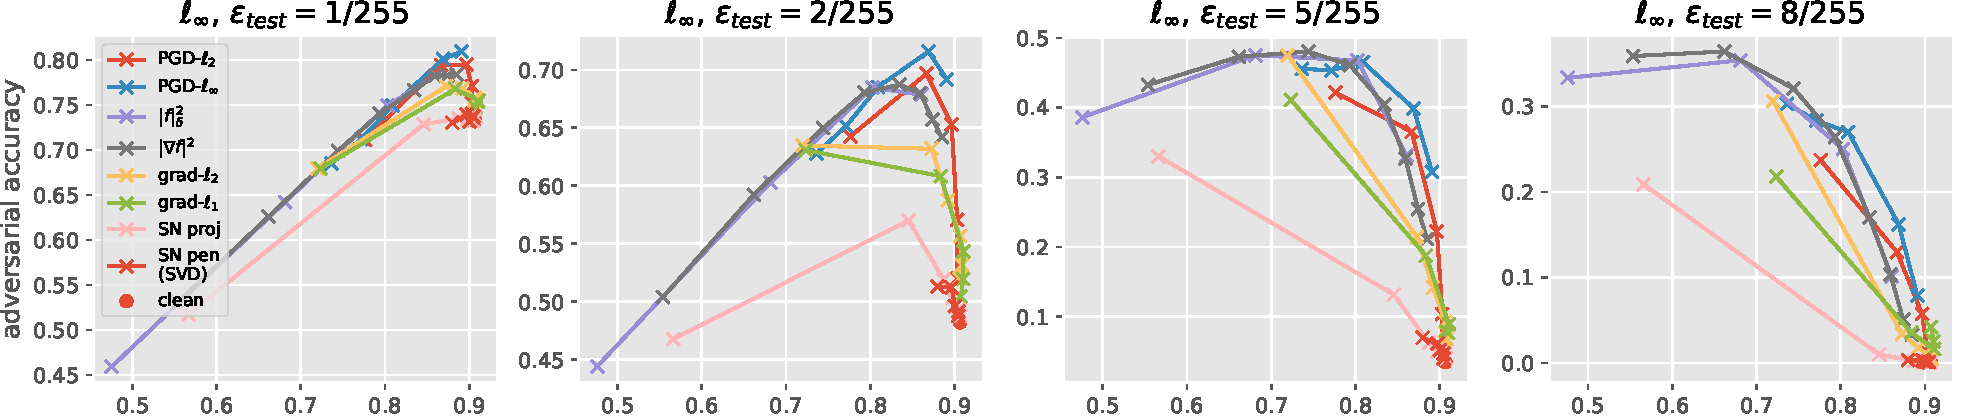
\includegraphics[width=.95\textwidth]{figures/cifar10_vgg/test_vs_adv_linf.pdf}
% 	\caption{$\ell_\infty$ robustness trade-off curves of different regularization methods for VGG11 on CIFAR10.
% 	Each plot shows test accuracy vs adversarial test accuracy
% 	for $\ell_\infty$ bounded 40-step PGD adversaries with a fixed~$\epsilon_{\text{test}}$.
% 	Different points on a curve correspond to training with different regularization strengths,
% 	with the leftmost points corresponding to the strongest regularization.}
% 	\label{fig:robust_tradeoffs_linf}
% \end{figure*}


\section{Details on Generalization Guarantees}
\label{sec:generalization_appx}
%!TEX root = main.tex

This section presents the proof of Proposition~\ref{prop:robust_margin_bound},
which relies on standard tools from statistical learning theory~\citep[\eg,][]{boucheron2005theory}.

\subsection{Proof of Proposition~\ref{prop:robust_margin_bound}}
\begin{proof}
Assume for now that~$\gamma$ is fixed in advance, and let $\mathcal F_\lambda := \{f \in \Hc : \|f\|_\Hc \leq \lambda\}$.
Note that for all~$f \in \mathcal F_\lambda$ we have
\begin{align*}
\text{err}_\mathcal{D}(f, \epsilon) = P(\exists \|\delta\| \leq \epsilon: y f(x + \delta) < 0) \leq P(yf(x) < \lambda \epsilon) =: L^{\lambda \epsilon}(f),
\end{align*}
since~$\|f\|_\Hc \leq \lambda$ is an upper bound on the Lipschitz constant of~$f$.
Consider the function
\begin{align*}
\phi(x) = \begin{cases}
	0, &\text{ if }x \leq -\gamma - \lambda \epsilon\\
	1, &\text{ if }x \geq - \lambda \epsilon\\
	1 + (x + \lambda \epsilon)/\gamma, &\text{ otherwise.}
\end{cases}
\end{align*}
Defining $A(f) = \E \phi(-y f(x)) \geq L^{\lambda \epsilon}(f)$ and $A_n(f) = \frac{1}{n} \sum_{i=1}^n \phi(- y_i f(x_i)) \leq L_n^{\lambda \epsilon + \gamma}(f)$,
and noting that $\phi$ is upper bounded by 1 and $1/\gamma$ Lipschitz,
we can apply similar arguments to~\citep[Theorem 4.1]{boucheron2005theory} to obtain,
with probability $1 - \delta$,
\begin{equation*}
L^\lambda \epsilon(f) \leq L_n^{\lambda \epsilon + \gamma}(f) + O \left(\frac{1}{\gamma} R_n(\mathcal{F}_\lambda) + \sqrt{\frac{\log 1/\delta}{n}} \right),
\end{equation*}
where~$R_n(\mathcal{F}_\lambda)$ denotes the empirical Rademacher complexity of~$\mathcal{F}_\lambda$ on the dataset $\{(x_i, y_i)\}_{i=1, \ldots, n}$.
Standard upper bounds on empirical Rademacher complexity of kernel classes with bounded RKHS norm yield the following bound
\begin{align*}
\text{err}_\mathcal{D}(f, \epsilon) \leq L_n^{\lambda \epsilon + \gamma}(f) + O \left( \frac{\lambda}{\gamma \sqrt{n}} \sqrt{\frac{1}{n}\sum_{i=1}^n K(x_i, x_i)} + \sqrt{\frac{\log 1/\delta}{n}} \right).
\end{align*}
Note that the bound is still valid with $\gamma' \geq \gamma$ instead of~$\gamma$ in the first term
of the r.h.s., since $L_n^{\gamma}(f)$ is non-decreasing as a function of~$\gamma$.

In order to establish the final bound, we instantiate the previous bound for values $\lambda_i = 2^i$ and $\gamma_j = 2^{-j}$.
Defining $\delta_{i,j} = \frac{\delta}{(1 + 4i^2) \cdot ( 1 + 4j^2)}$, we have that w.p. $1 - \delta_{i,j}$, for all $f \in \mathcal F_{\lambda_i}$ and all $\gamma \geq \gamma_j$,

\begin{align}
\label{eq:bound_single}
\text{err}_\mathcal{D}(f, \epsilon) \leq L_n^{\lambda_i \epsilon + \gamma}(f) + O \left( \frac{\lambda_i}{\gamma_j \sqrt{n}} \sqrt{\frac{1}{n}\sum_{i=1}^n K(x_i, x_i)} + \sqrt{\frac{\log 1/\delta_{i,j}}{n}} \right).
\end{align}
By a union bound, this event holds jointly for all integers $i, j$ w.p. greater than $1 - \delta$,
since $\sum_{i,j} \delta_{i,j} \leq \delta$.
Now consider an arbitrary $f \in \Hc$ and $\gamma > 0$ and let $i = \lceil \log_2 \|f\|_\Hc \rceil$
and $j = \lceil \log_2 (1/\gamma) \rceil$. We have
\begin{align*}
\lambda_i &\leq 2 \|f\|_\Hc \\
\frac{1}{\gamma_j} &\leq \frac{2}{\gamma} \\
\log(1/\delta_{i,j}) &\leq \log(C(\|f\|_\Hc, \gamma) / \delta),
\end{align*}
with $C(\|f\|_\Hc, \gamma) := (1 + 4(\log_2\|f\|_\Hc)^2) \cdot (1 + 4(\log_2 (1/\gamma))^2)$.
Applying this to the bound in~\eqref{eq:bound_single} yields the desired result.

\end{proof}


\end{document}
